\section{Hypothèse sur les coûts : « \textit{combien dois-je investir ?} »}
\label{section:4.3-HYPOTHESE-COUTS}

	%%% Formulation des hypothèses:
	Pour compléter l'étude réalisée sur l'hypothèse d'efficience (optimisation des paramètres de convergence, cf. section~\ref{section:4.3-HYPOTHESE-EFFICIENCE}), nous aimerions vérifier l'hypothèse suivante :
	\todo{à compléter}

	\begin{tcolorbox}[
		title=\faVial~\textbf{Hypothèse sur les coûts}~\faVial,
		colback=colorTcolorboxHypothesis!15,
		colframe=colorTcolorboxHypothesis!75,
		width=\linewidth
	]
		% Hypothèse.
		«\textbf{
			Il est possible d'\textbf{estimer les coûts nécessaires} d'une méthodologie d'annotation basée sur le \textit{clustering} interactif pour obtenir une base d'apprentissage exploitable. Nous étudierons en particulier les coûts relatifs au temps d'annotation, au temps de calculs des algorithmes, ainsi que la durée totale de la méthode en fonction de la taille du jeu de données.
		} » \\

		% Résumé de l'étude.
		Afin de vérifier cette hypothèse, nous organiserons plusieurs expériences pour simuler ou déterminer ces durées en fonction de plusieurs facteurs : taille du jeu de données, nombre de clusters, nombre de contraintes, différents annotateurs, ...
		
		% Figure.
		La figure~\ref{figure:4.3-HYPOTHESE-COUTS} illustre cette hypothèse et l'espoir de pouvoir caractériser la qualité de la base d'apprentissage en cours de construction en fonction d'un coût temporel au lieu d'un nombre abstrait d'itérations de la méthode. 
		%
		
		\begin{figure}[H]  % keep [H] to be in the tcolorbox.
			\centering
			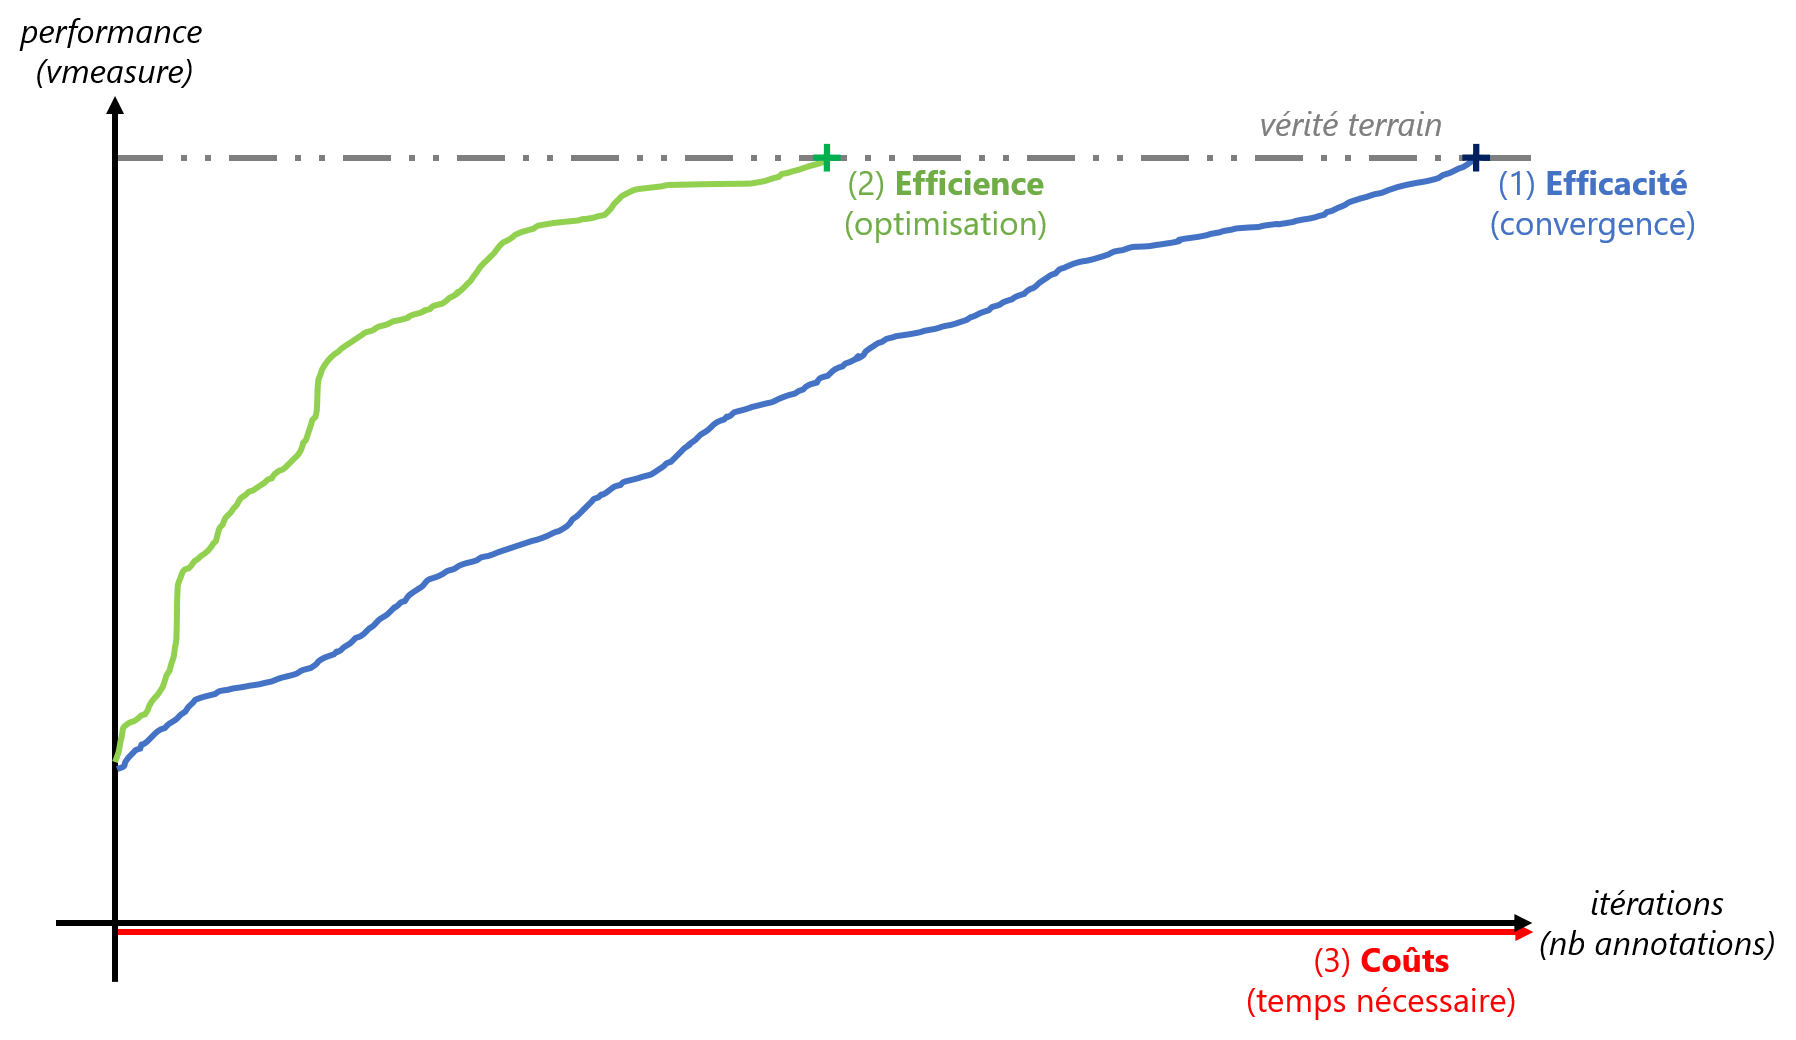
\includegraphics[width=0.8\textwidth]{figures/hypotheses-03-couts}
			\caption{Illustration des études réalisées sur le \textit{clustering} interactif (\textit{étape 3/6}) en schématisant l'évolution de la performance (\textit{accord avec la vérité terrain calculé en v-measure}) d'une base d'apprentissage en cours de construction en fonction du nombre d'itérations de la méthode (\textit{nombre d'annotations par un expert métier}).}
			\label{figure:4.3-HYPOTHESE-COUTS}
		\end{figure}

	\end{tcolorbox}
	

	%%%
	%%% Subsection 4.3.1: Étude d'estimation du temps de calcul des algorithmes
	%%%
	\subsection{Étude d'estimation du temps de calcul des algorithmes}
	\label{section:4.3.1-HYPOTHESE-COUTS-TEMPS-CALCUL}
	
		%%% Protocole expérimental.
		\subsubsection{Protocole expérimental}
		
			% Objectif de l'expérience.
			% Détails de l'expérience.
			% Description des tâches, des algorithmes et des paramètres.
			\todo[inline]{A REDIGER: Protocole + Données + Critères}

		%%% Résultats
		\subsubsection{Résultats obtenus}
		
			% Prétraitements
			\todo[inline]{A REDIGER: Description figure}
			\begin{figure}[!htb]
				\centering
				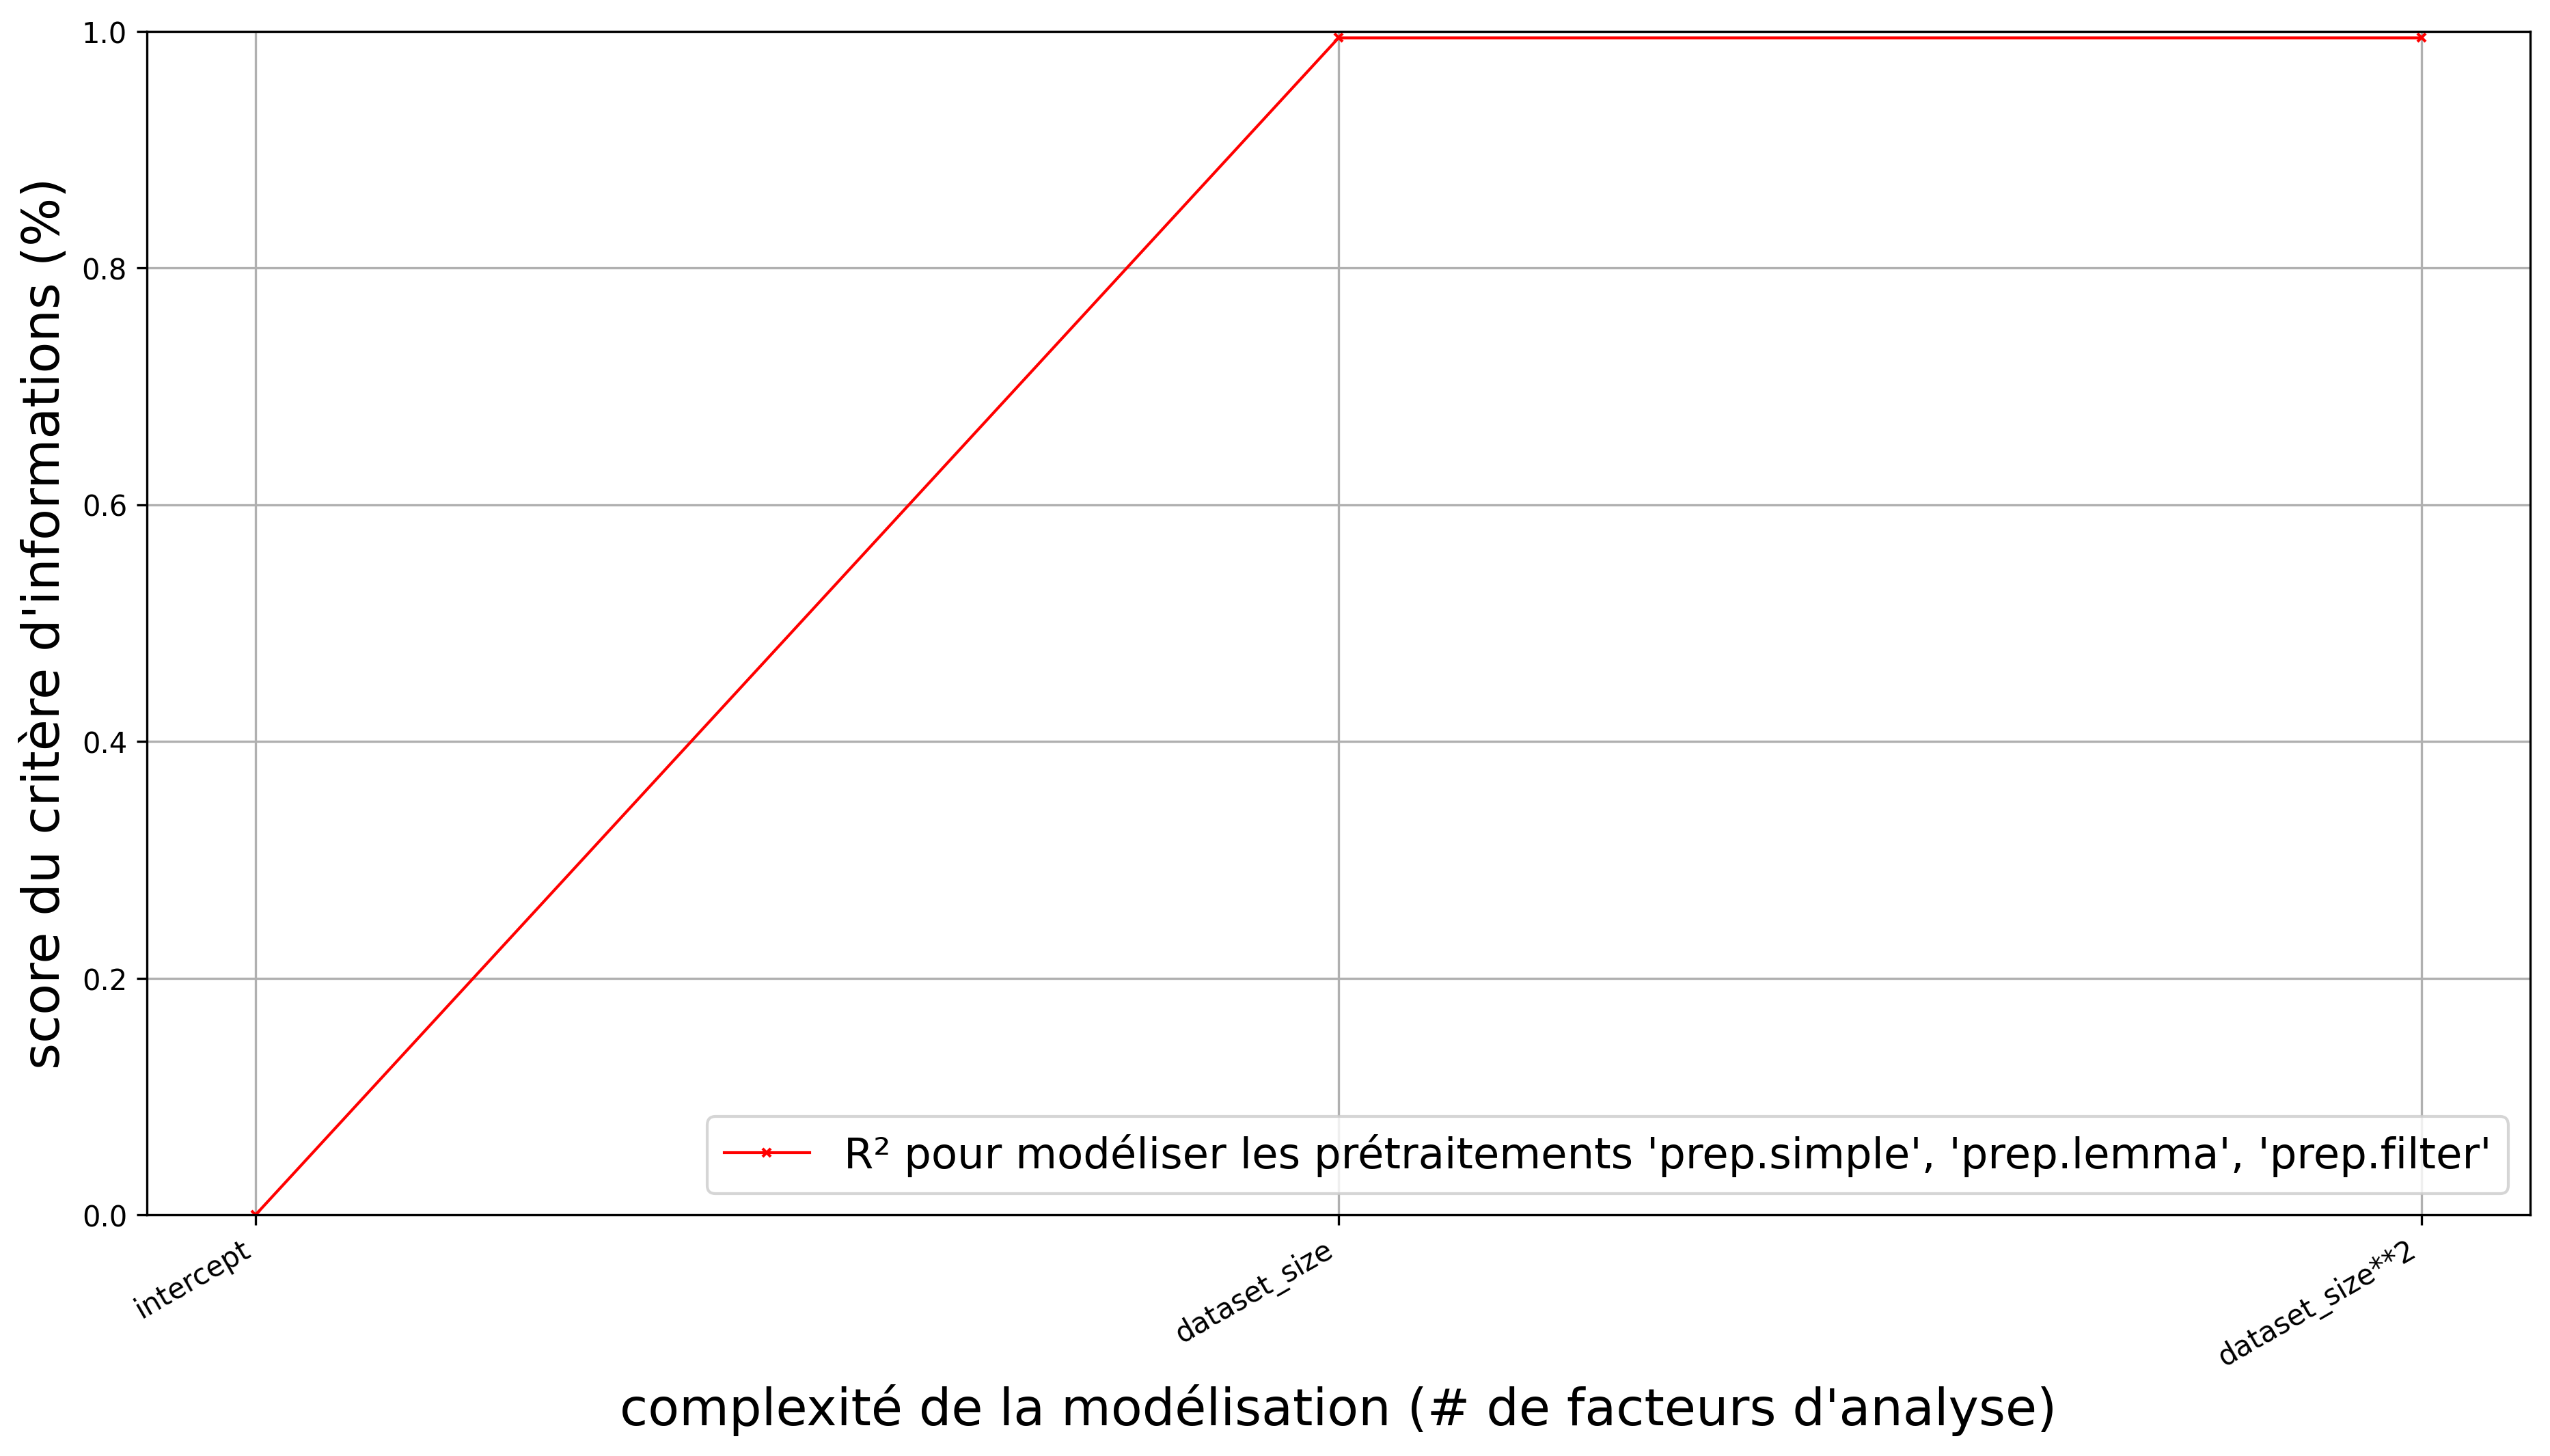
\includegraphics[width=\textwidth]{figures/etude-temps-calcul-analyse-facteurs-1prep}
				\caption{Évolution de score d'information (en \(R^2\)) caractérisant une modélisation du temps de calcul de la tâche de \textbf{prétraitement} en fonction du degré de complexité (basé sur les interactions entre les facteurs d'analyse suivants : \textbf{(a)} \texttt{nombre de données}. Les paramétrages \texttt{prep.simple}, \texttt{prep.lemma} et \texttt{prep.filter} ayant des temps de calculs similaires, leurs modélisations n'ont pas été séparées.}
				\label{figure:4.3.1-ETUDE-COUTS-TEMPS-CALCUL-ANALYSE-FACTEURS-PREPROCESSING}
			\end{figure}
		
			\todo[inline]{A REDIGER: Description figure}
			\begin{figure}[!htb]
				\centering
				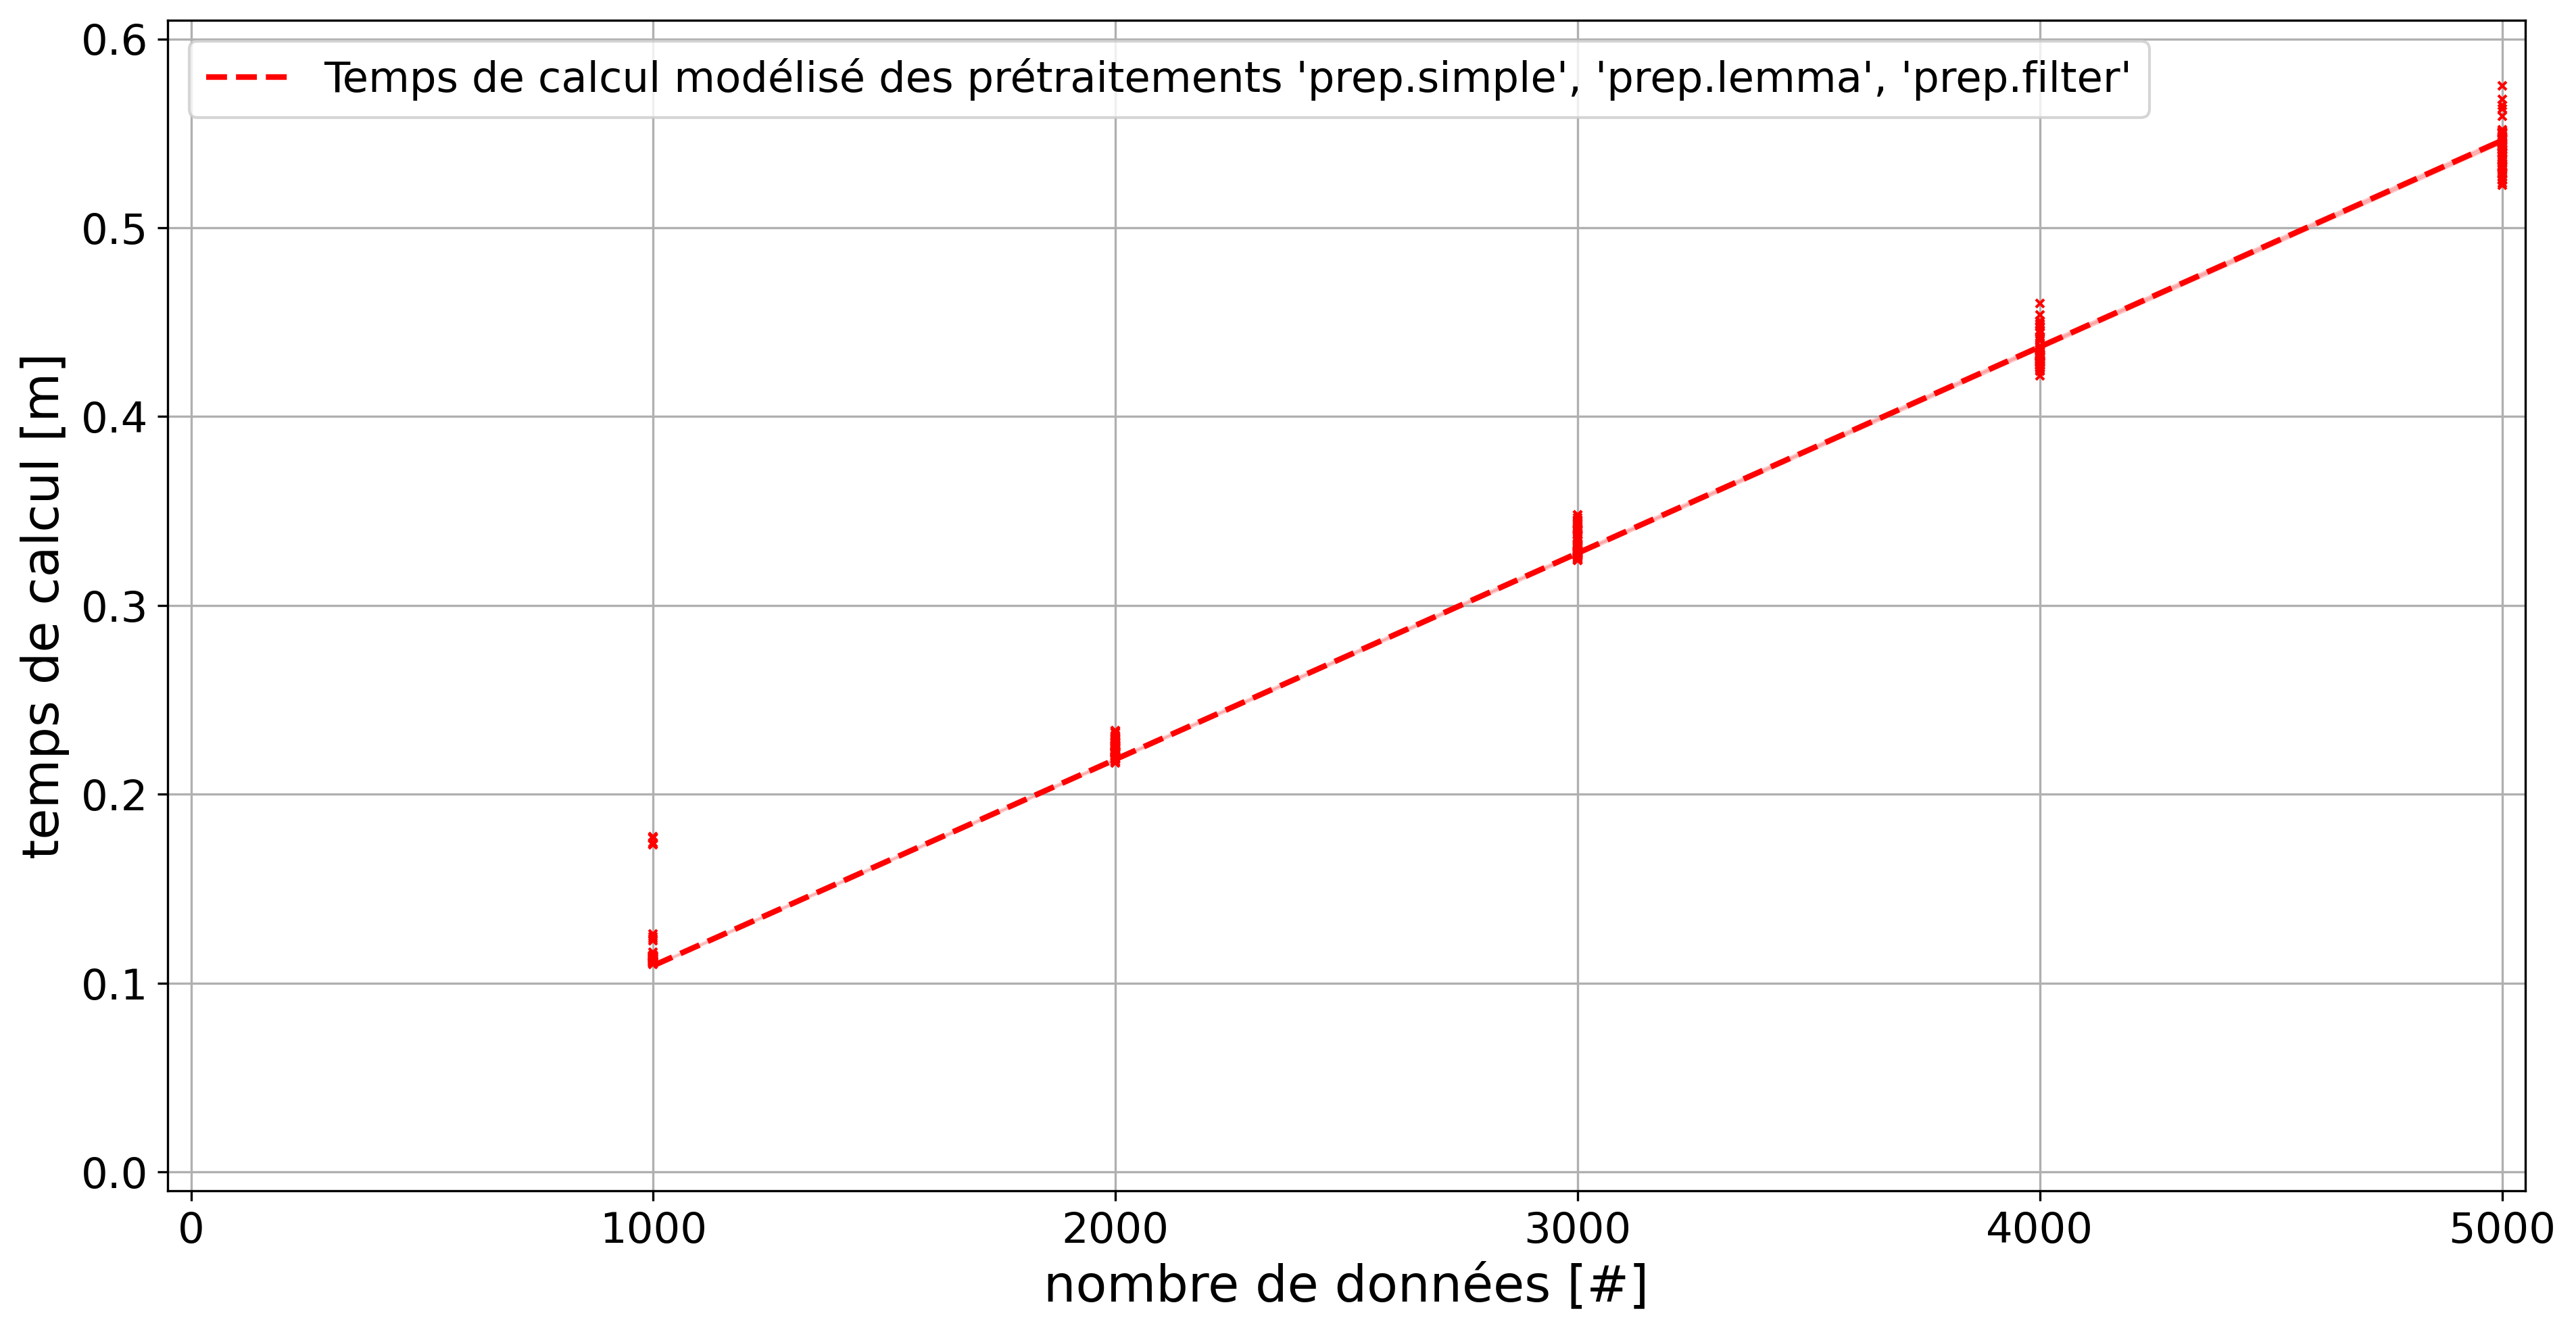
\includegraphics[width=\textwidth]{figures/etude-temps-calcul-modelisation-1prep}
				\caption{Estimation du temps nécessaire (en secondes) pour effectuer une tâche de \textbf{prétraitement} en fonction du nombre de données à traiter. Les paramétrages \texttt{prep.simple}, \texttt{prep.lemma} et \texttt{prep.filter} ayant des temps de calculs similaires, leurs modélisations n'ont pas été séparées.}
				\label{figure:4.3.1-ETUDE-COUTS-TEMPS-CALCUL-MODELISATION-PREPROCESSING}
			\end{figure}
			
			\todo[inline]{A REDIGER: Equation}
			
			% Vectorization
			\todo[inline]{A REDIGER: Description figure}
			\begin{figure}[!htb]
				\centering
				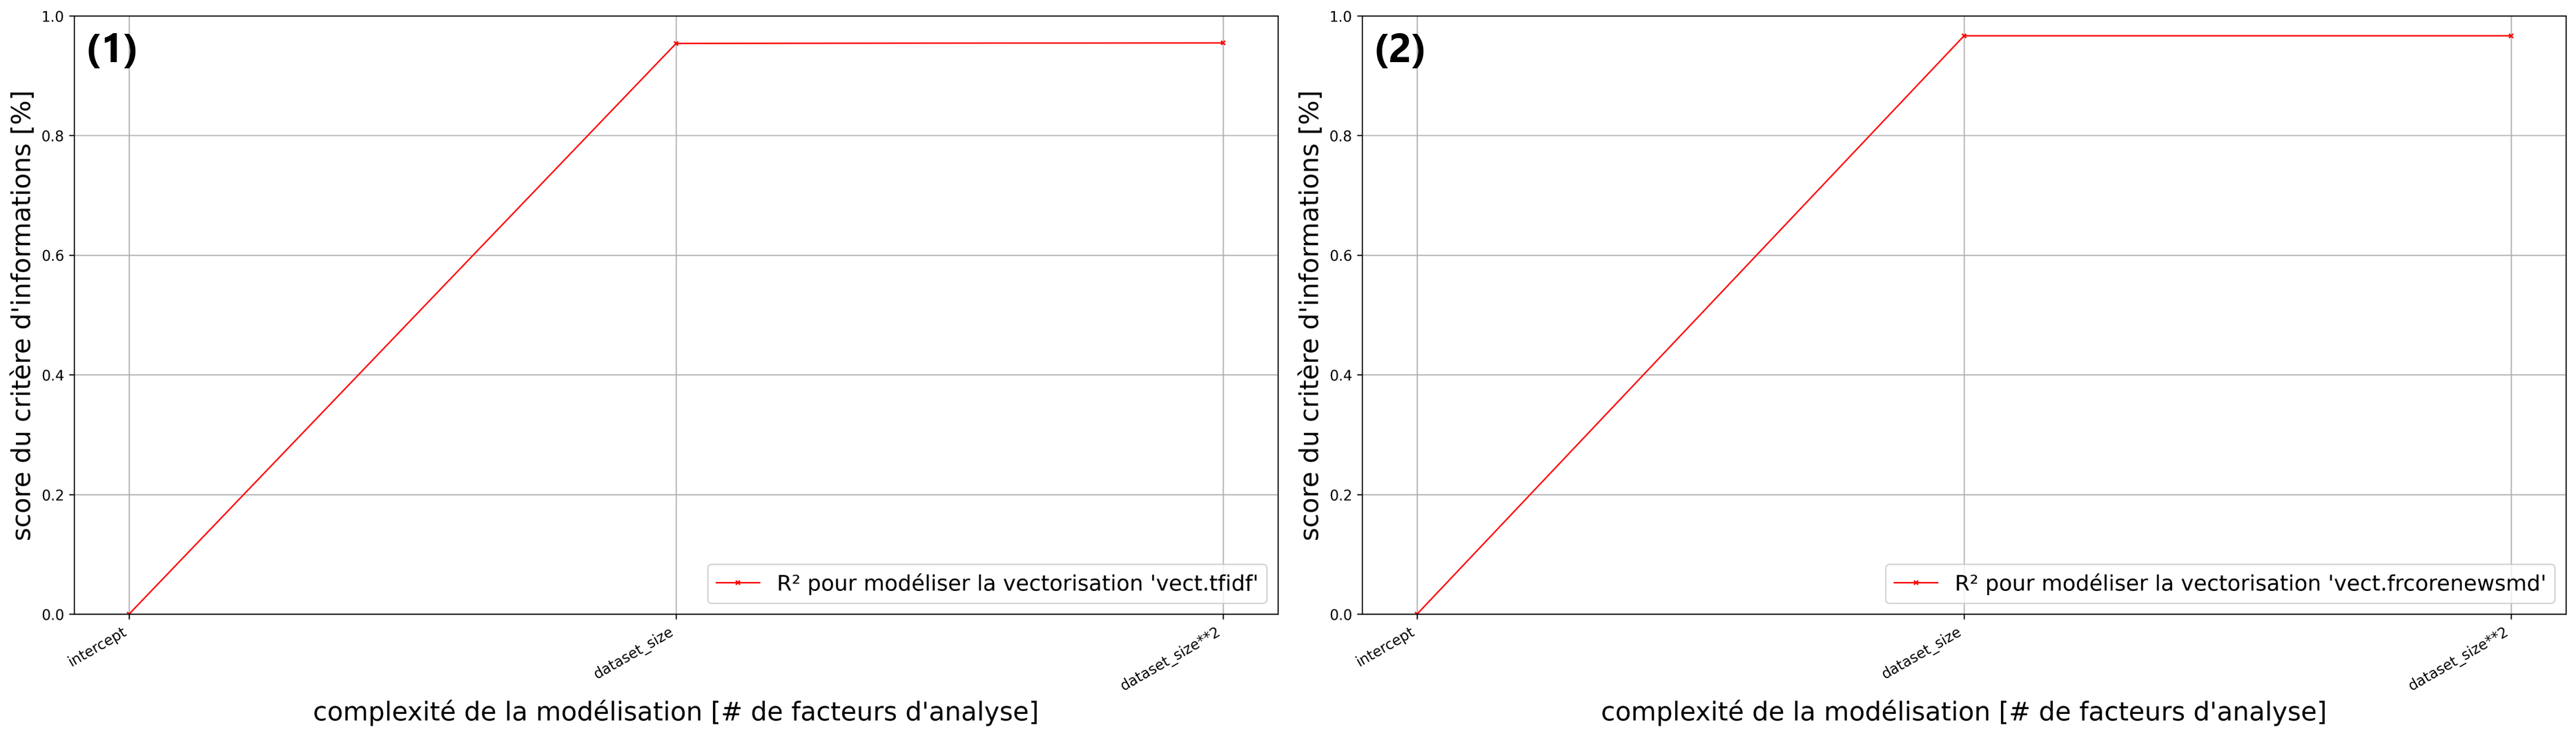
\includegraphics[width=\textwidth]{figures/etude-temps-calcul-analyse-facteurs-2vect}
				\caption{Évolution de score d'information (en \(R^2\)) caractérisant une modélisation du temps de calcul de la tâche de \textbf{vectorisation} en fonction du degré de complexité (basé sur les interactions entre les facteurs d'analyse suivants : \textbf{(a)} \texttt{nombre de données}. Au sujet de la correspondance des graphes : \textbf{(1)}=\texttt{vect.tfidf} ; \textbf{(2)}=\texttt{vect.frcorenewsmd}.}
				\label{figure:4.3.1-ETUDE-COUTS-TEMPS-CALCUL-ANALYSE-FACTEURS-VECTORIZATION}
			\end{figure}
		
			\todo[inline]{A REDIGER: Description figure}
			\begin{figure}[!htb]
				\centering
				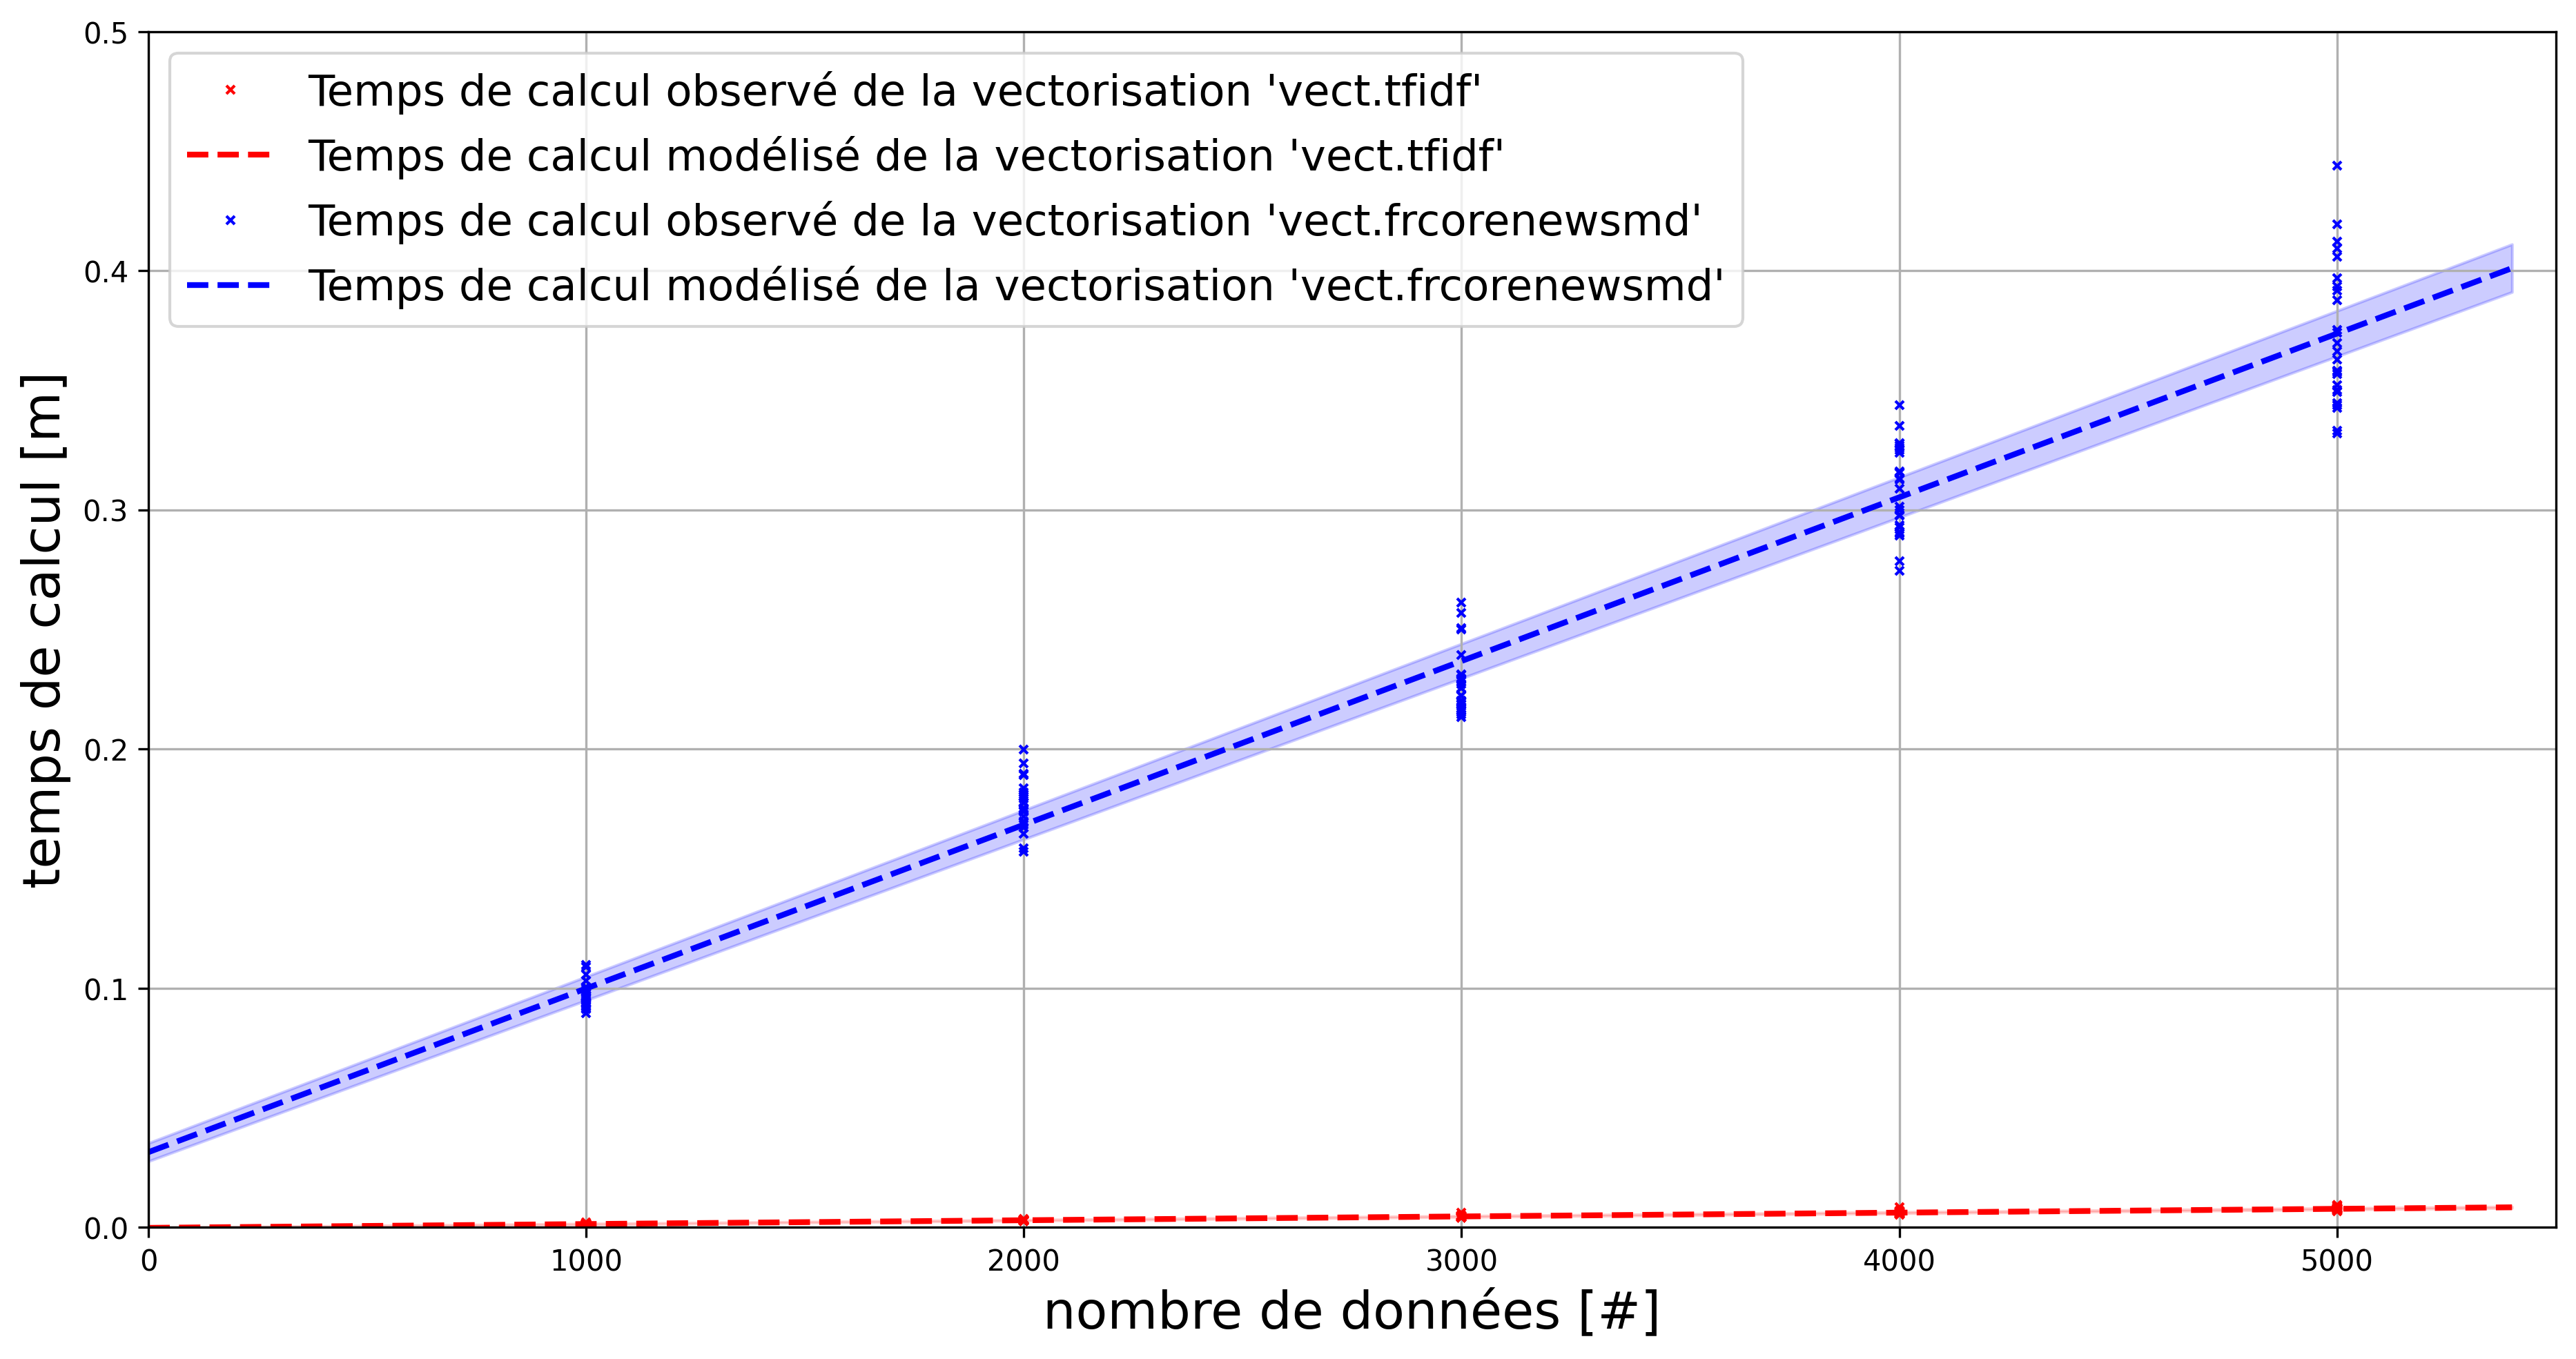
\includegraphics[width=\textwidth]{figures/etude-temps-calcul-modelisation-2vect}
				\caption{Estimation du temps nécessaire (en secondes) pour effectuer une tâche de \textbf{vectorisation} en fonction du nombre de données à traiter.}
				\label{figure:4.3.1-ETUDE-COUTS-TEMPS-CALCUL-MODELISATION-VECTORIZATION}
			\end{figure}
			
			\todo[inline]{A REDIGER: Equation}
			
			% Vectorization
			\todo[inline]{A REDIGER: Description figure}
			\begin{figure}[!htb]
				\centering
				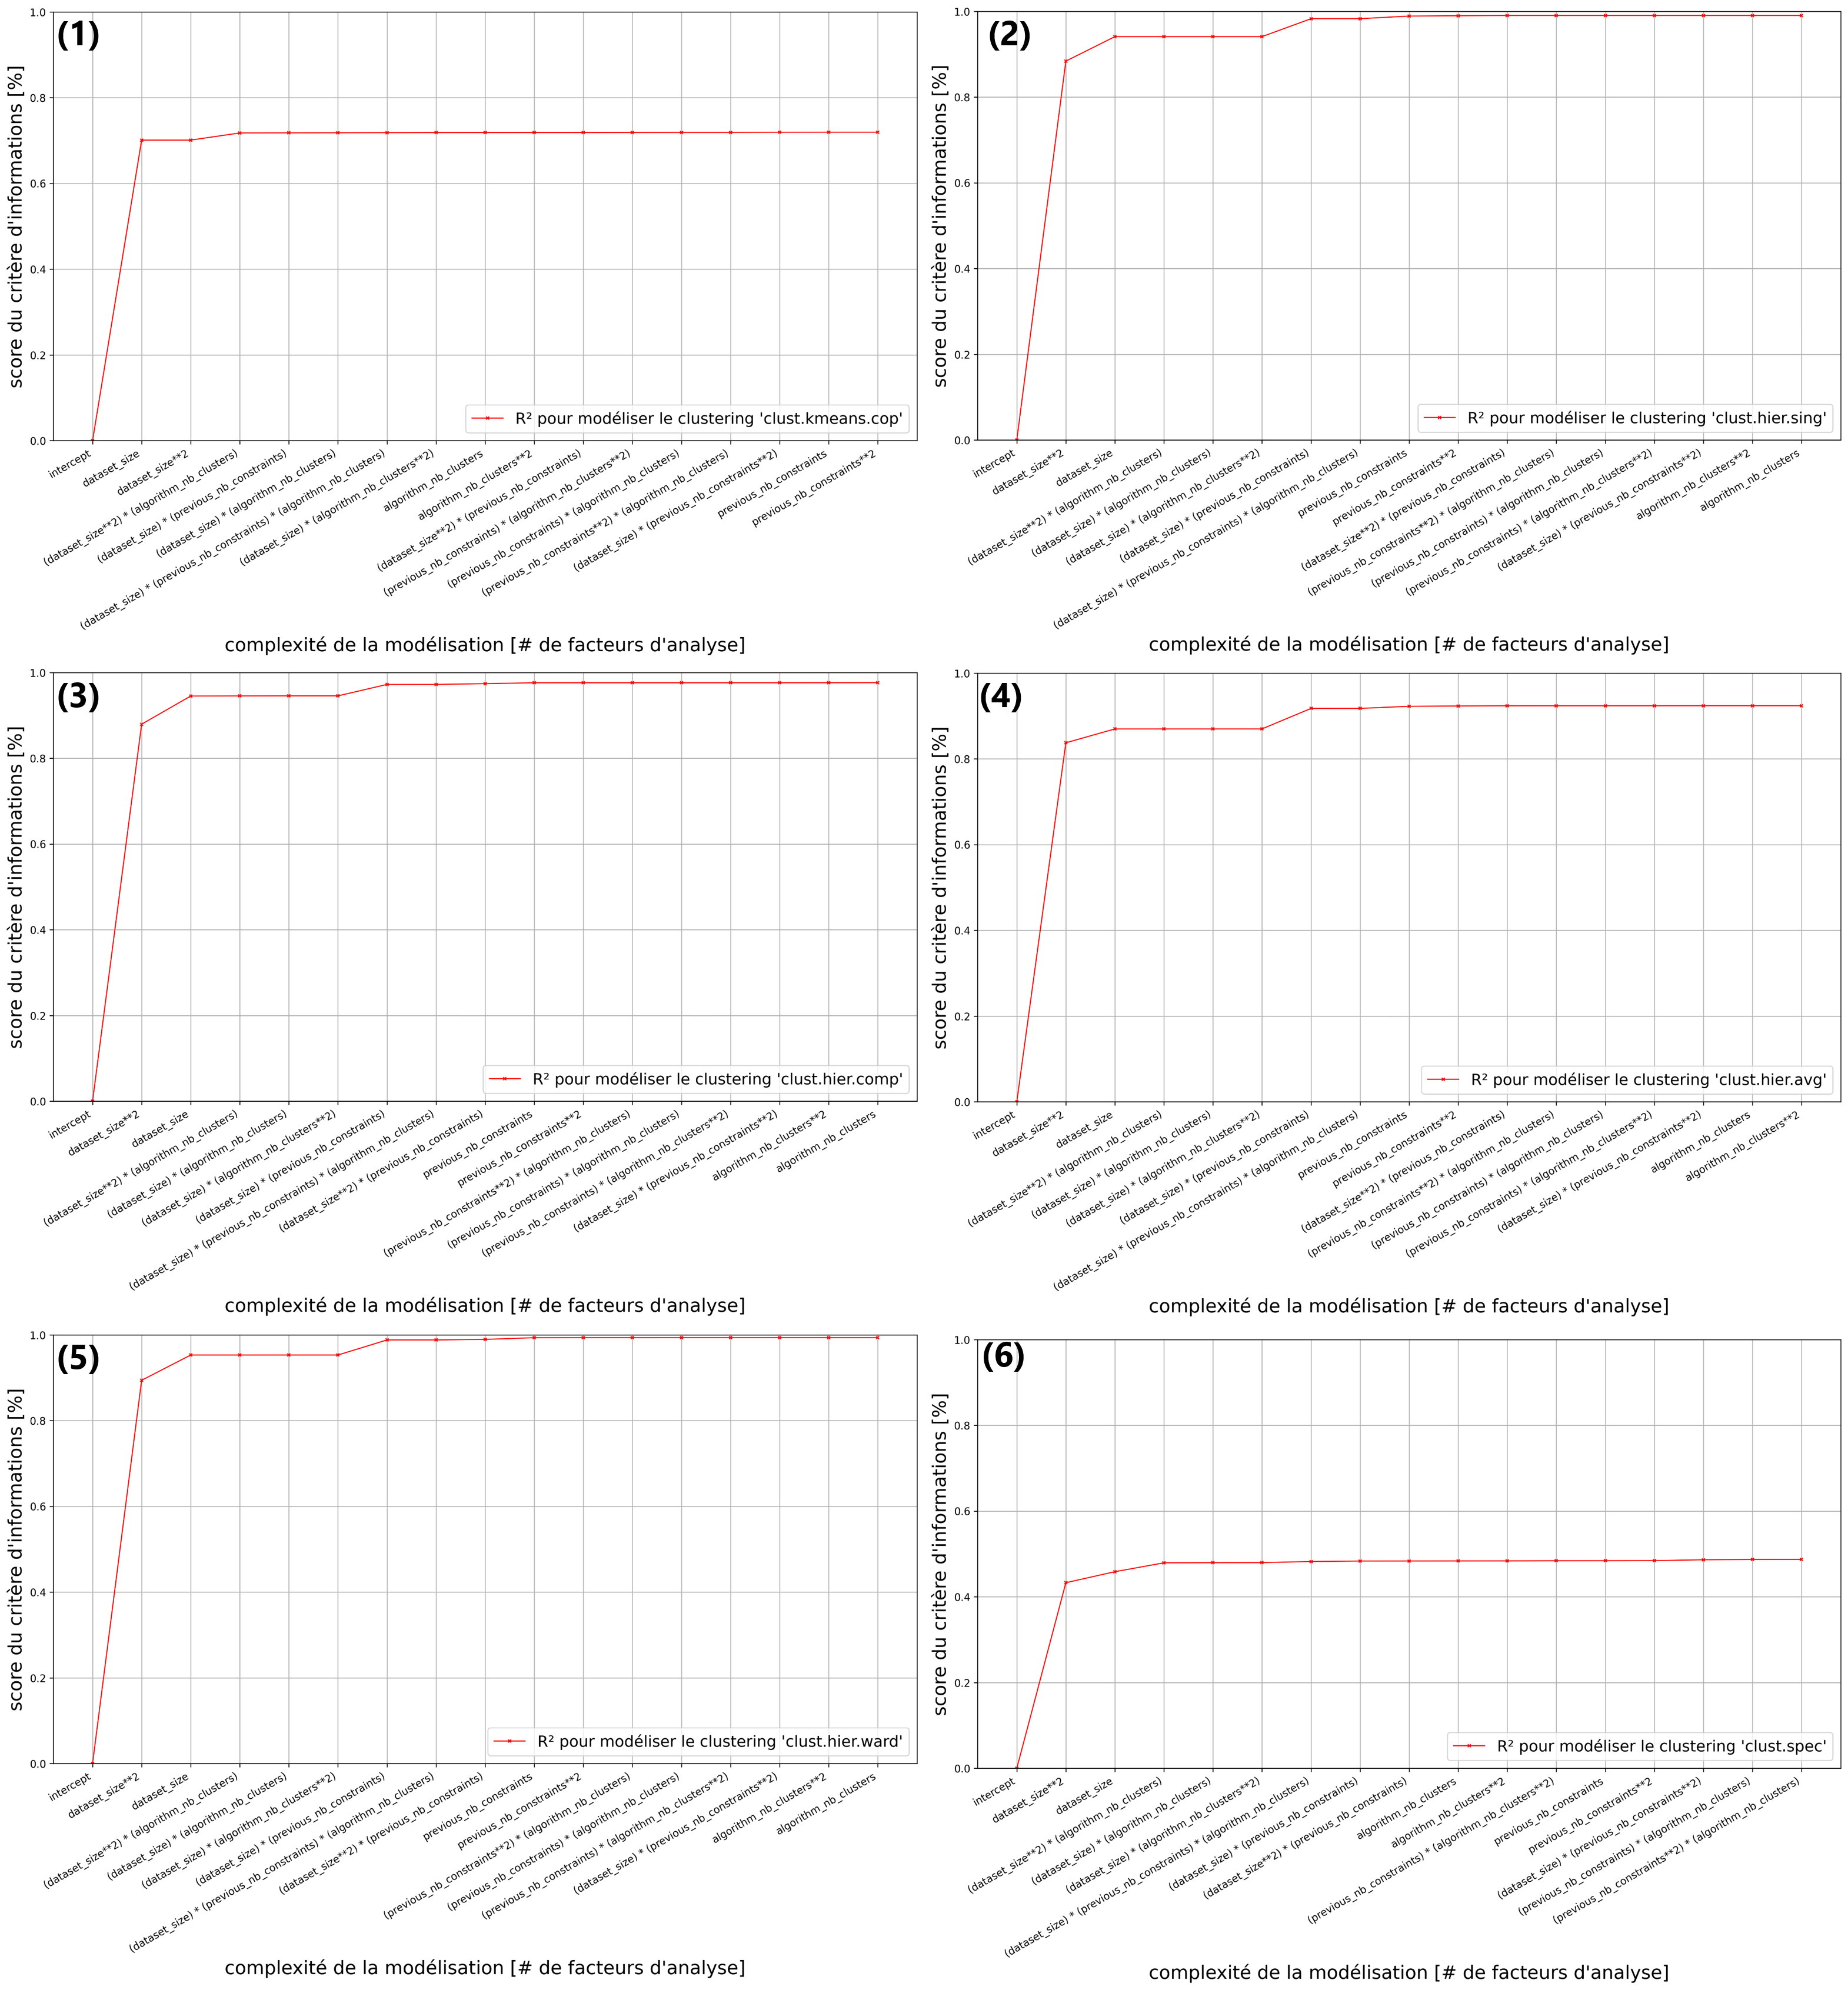
\includegraphics[width=\textwidth]{figures/etude-temps-calcul-analyse-facteurs-3clust}
				\caption{Évolution de score d'information (en \(R^2\)) caractérisant une modélisation du temps de calcul de la tâche de \textbf{clustering} en fonction du degré de complexité (basé sur les interactions entre les facteurs d'analyse suivants : \textbf{(a)} \texttt{nombre de données}, \textbf{(b)} \texttt{nombre de clusters à trouver}, \textbf{(c)} \texttt{nombre contraintes annotées}. Au sujet de la correspondance des graphes : \textbf{(1)}=\texttt{clust.kmeans.cop} ; \textbf{(2)}=\texttt{clust.hier.sing} ; \textbf{(3)}=\texttt{clust.hier.comp} ; \textbf{(4)}=\texttt{clust.hier.avg} ; \textbf{(5)}=\texttt{clust.hier.ward} ; \textbf{(6)}=\texttt{clust.spec}.}
				\label{figure:4.3.1-ETUDE-COUTS-TEMPS-CALCUL-ANALYSE-FACTEURS-CLUSTERING}
			\end{figure}
		
			\todo[inline]{A REDIGER: Description figure}
			\begin{figure}[!htb]
				\centering
				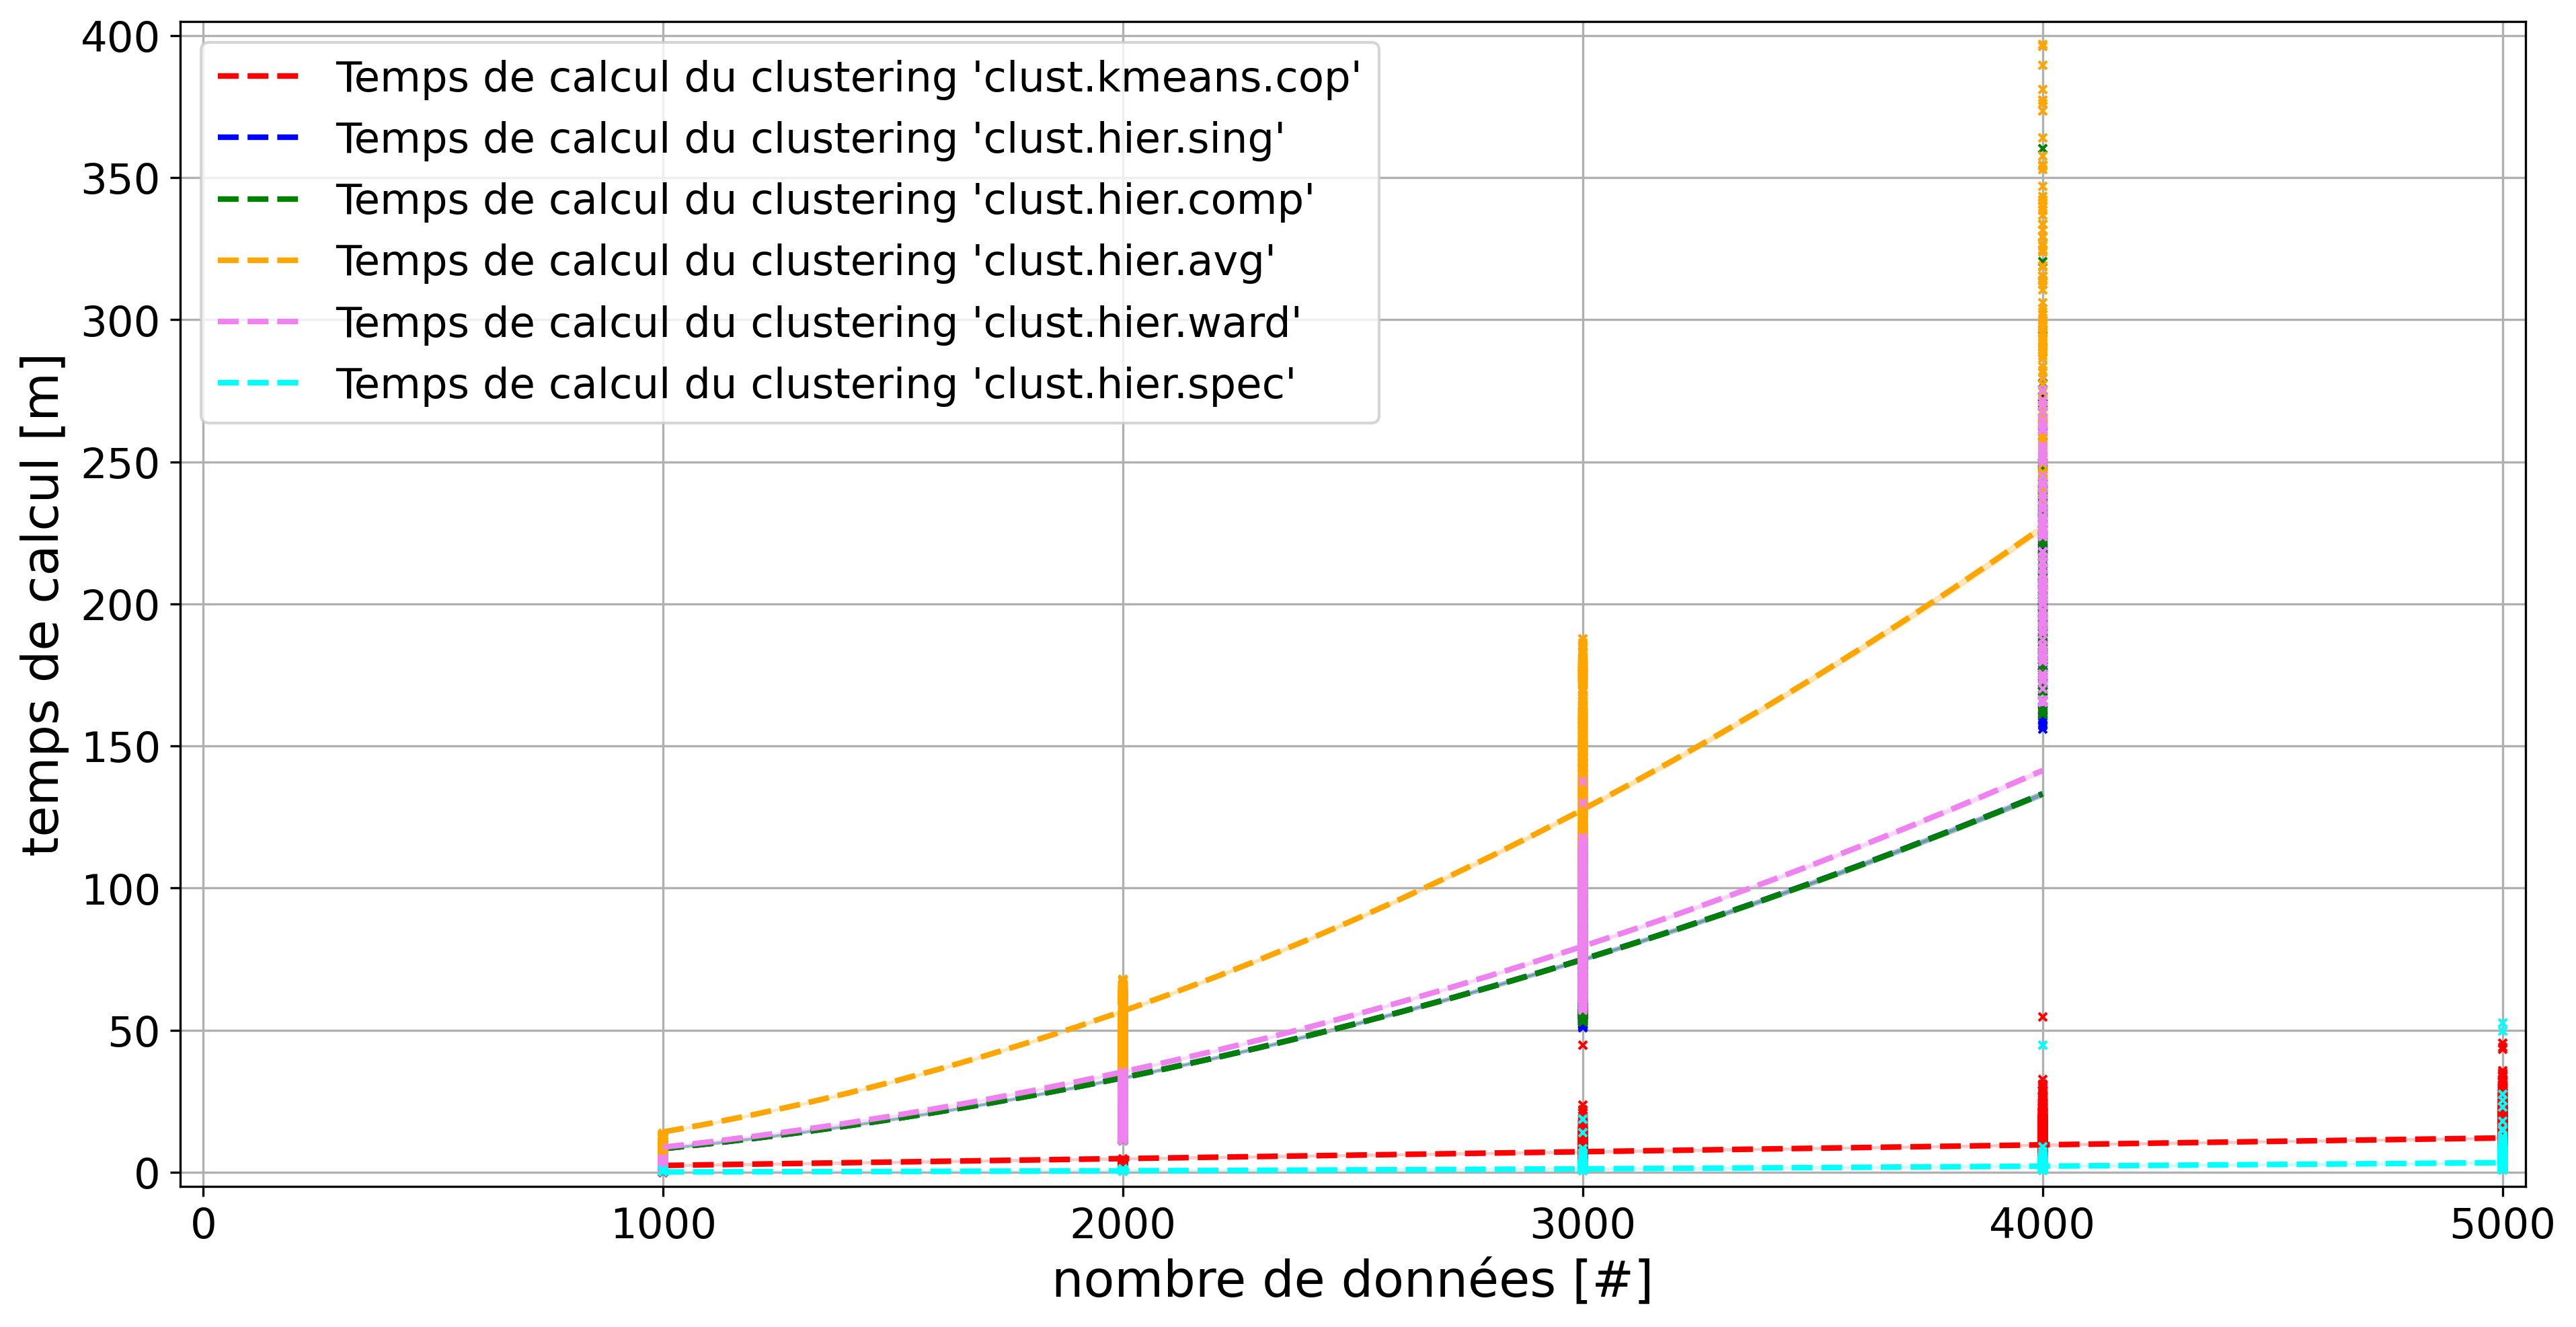
\includegraphics[width=\textwidth]{figures/etude-temps-calcul-modelisation-3clust}
				\caption{Estimation du temps nécessaire (en secondes) pour effectuer une tâche de \textbf{clustering} en fonction du nombre de données à traiter.}
				\label{figure:4.3.1-ETUDE-COUTS-TEMPS-CALCUL-MODELISATION-CLUSTERING}
			\end{figure}
			
			\todo[inline]{A REDIGER: Equation}
			
			% Vectorization
			\todo[inline]{A REDIGER: Description figure}
			\begin{figure}[!htb]
				\centering
				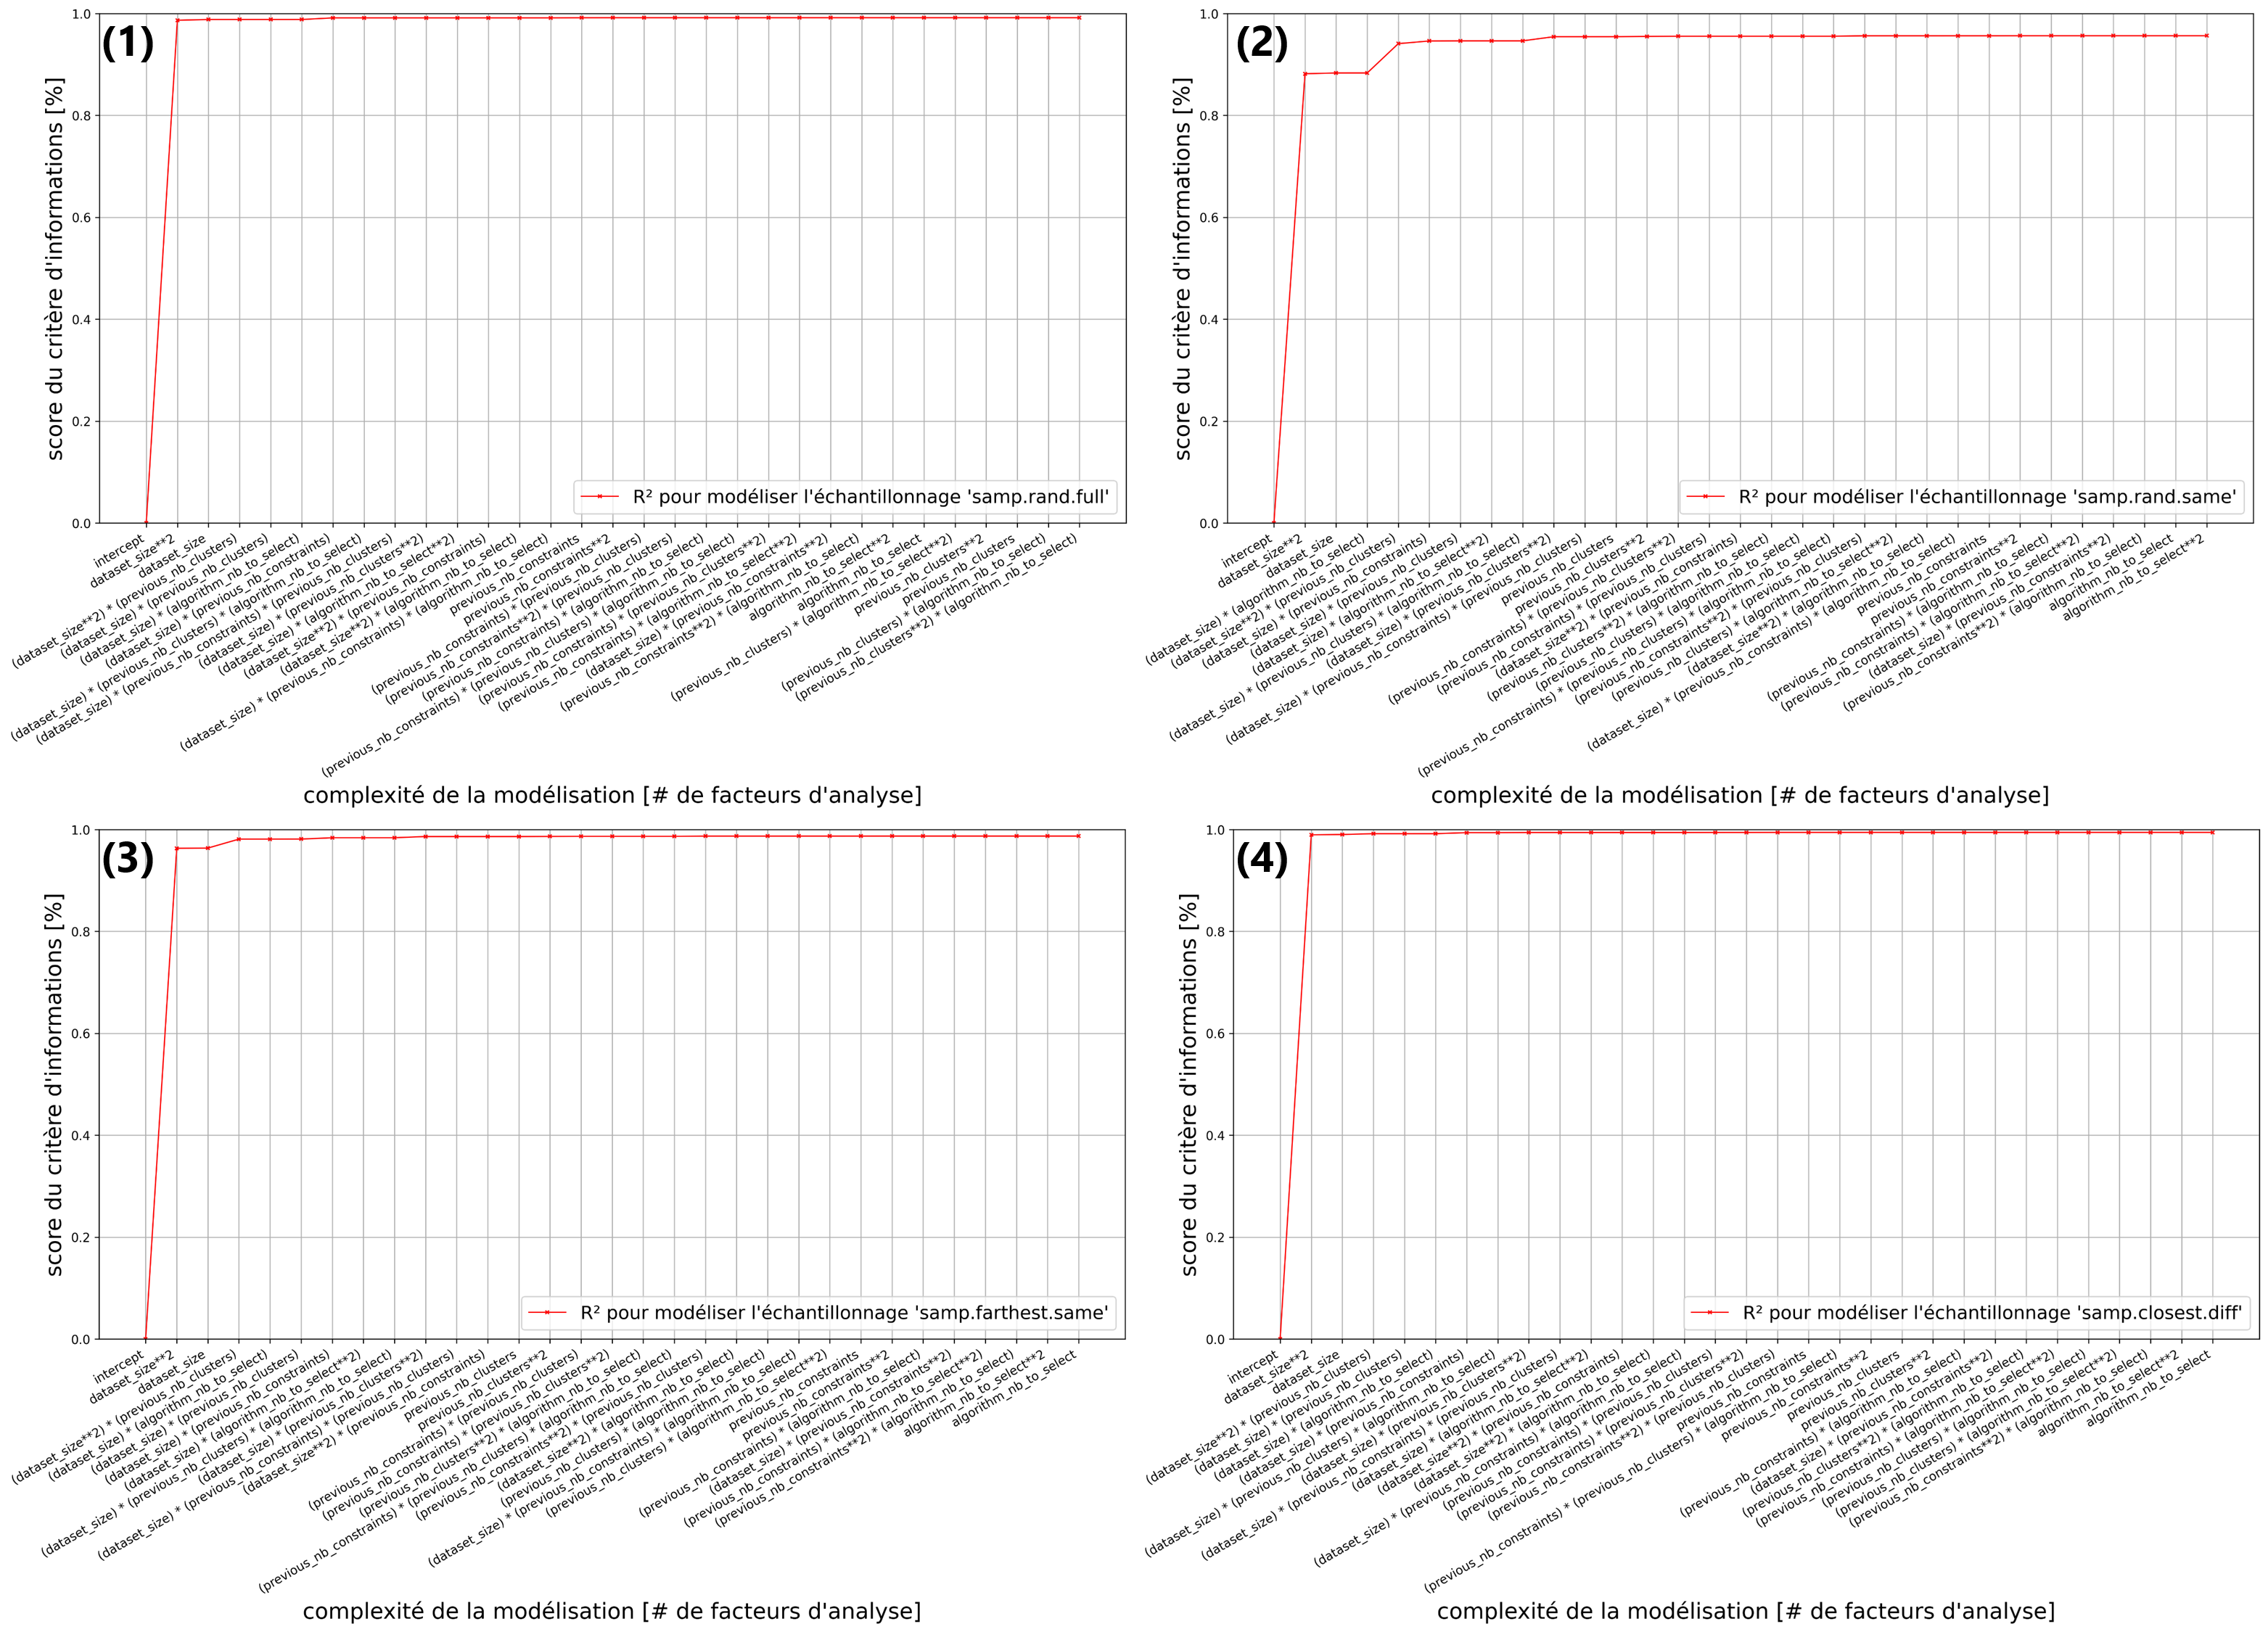
\includegraphics[width=\textwidth]{figures/etude-temps-calcul-analyse-facteurs-4samp}
				\caption{Évolution de score d'information (en \(R^2\)) caractérisant une modélisation du temps de calcul de la tâche d'\textbf{échantillonnage} en fonction du degré de complexité (basé sur les interactions entre les facteurs d'analyse suivants : \textbf{(a)} \texttt{nombre de données}, \textbf{(b)} \texttt{nombre de clusters}, \textbf{(c)} \texttt{nombre contraintes annotées}, \textbf{(d)} \texttt{nombre contraintes à sélectionner}. Au sujet de la correspondance des graphes : \textbf{(1)}=\texttt{samp.rand.full} ; \textbf{(2)}=\texttt{samp.rand.same} ; \textbf{(3)}=\texttt{clust.farthest.same} ; \textbf{(4)}=\texttt{clust.closest.diff}.}
				\label{figure:4.3.1-ETUDE-COUTS-TEMPS-CALCUL-ANALYSE-FACTEURS-SAMPLING}
			\end{figure}
		
			\todo[inline]{A REDIGER: Description figure}
			\begin{figure}[!htb]
				\centering
				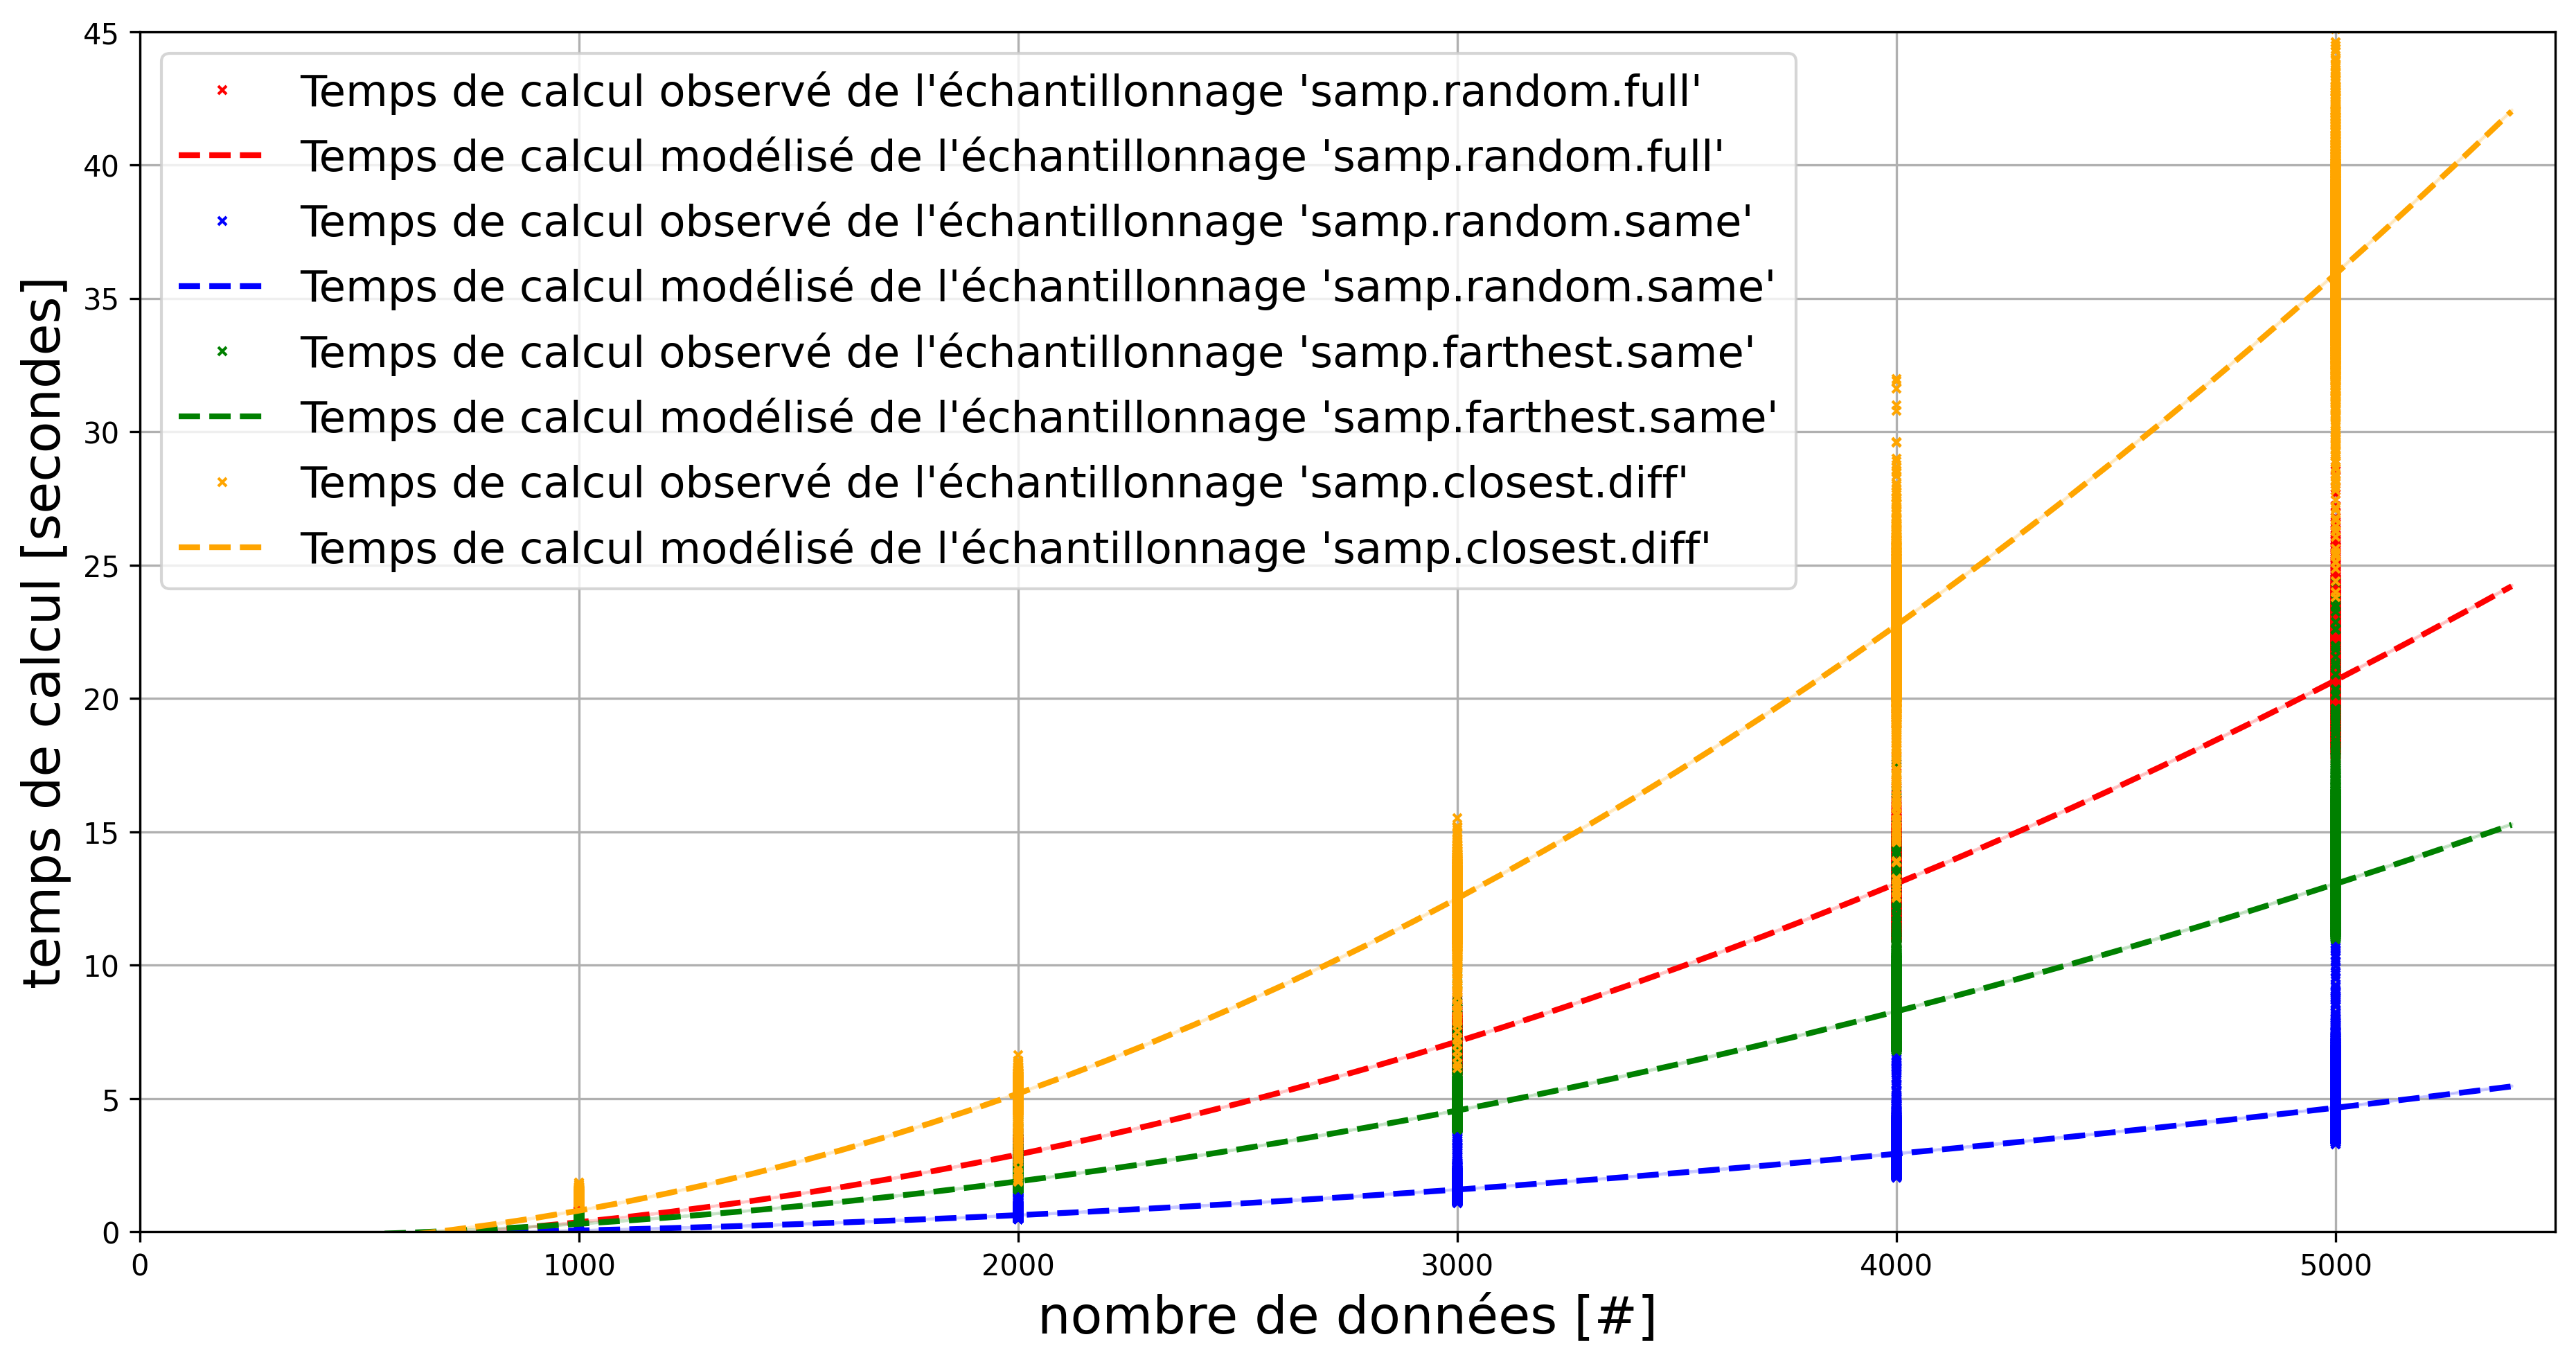
\includegraphics[width=\textwidth]{figures/etude-temps-calcul-modelisation-4samp}
				\caption{Estimation du temps nécessaire (en secondes) pour effectuer une tâche d'\textbf{échantillonnage} en fonction du nombre de données à traiter.}
				\label{figure:4.3.1-ETUDE-COUTS-TEMPS-CALCUL-MODELISATION-SAMPLING}
			\end{figure}
			
			\todo[inline]{A REDIGER: Equation}

		%%% Discussion
		\subsubsection{Discussion}
		
			\todo[inline]{A REDIGER: Discussion}
	
	%%%
	%%% Subsection 4.3.2: Étude d'estimation du temps d'annotation par un expert métier
	%%%
	\subsection{Étude d'estimation du temps d'annotation par un expert métier}
	\label{section:4.3.2-HYPOTHESE-COUTS-TEMPS-ANNOTATION}
	
		%%% Protocole expérimental.
		\subsubsection{Protocole expérimental}
		
			\todo[inline]{Description succincte du protocole expérimental dans l'encadré d'hypothèse ?}							\todo[inline]{A REDIGER: Protocole + Données + Critères}

		%%% Résultats
		\subsubsection{Résultats obtenus}
		
			\todo[inline]{A REDIGER: Description figure}
			\begin{figure}[!htb]
				\centering
				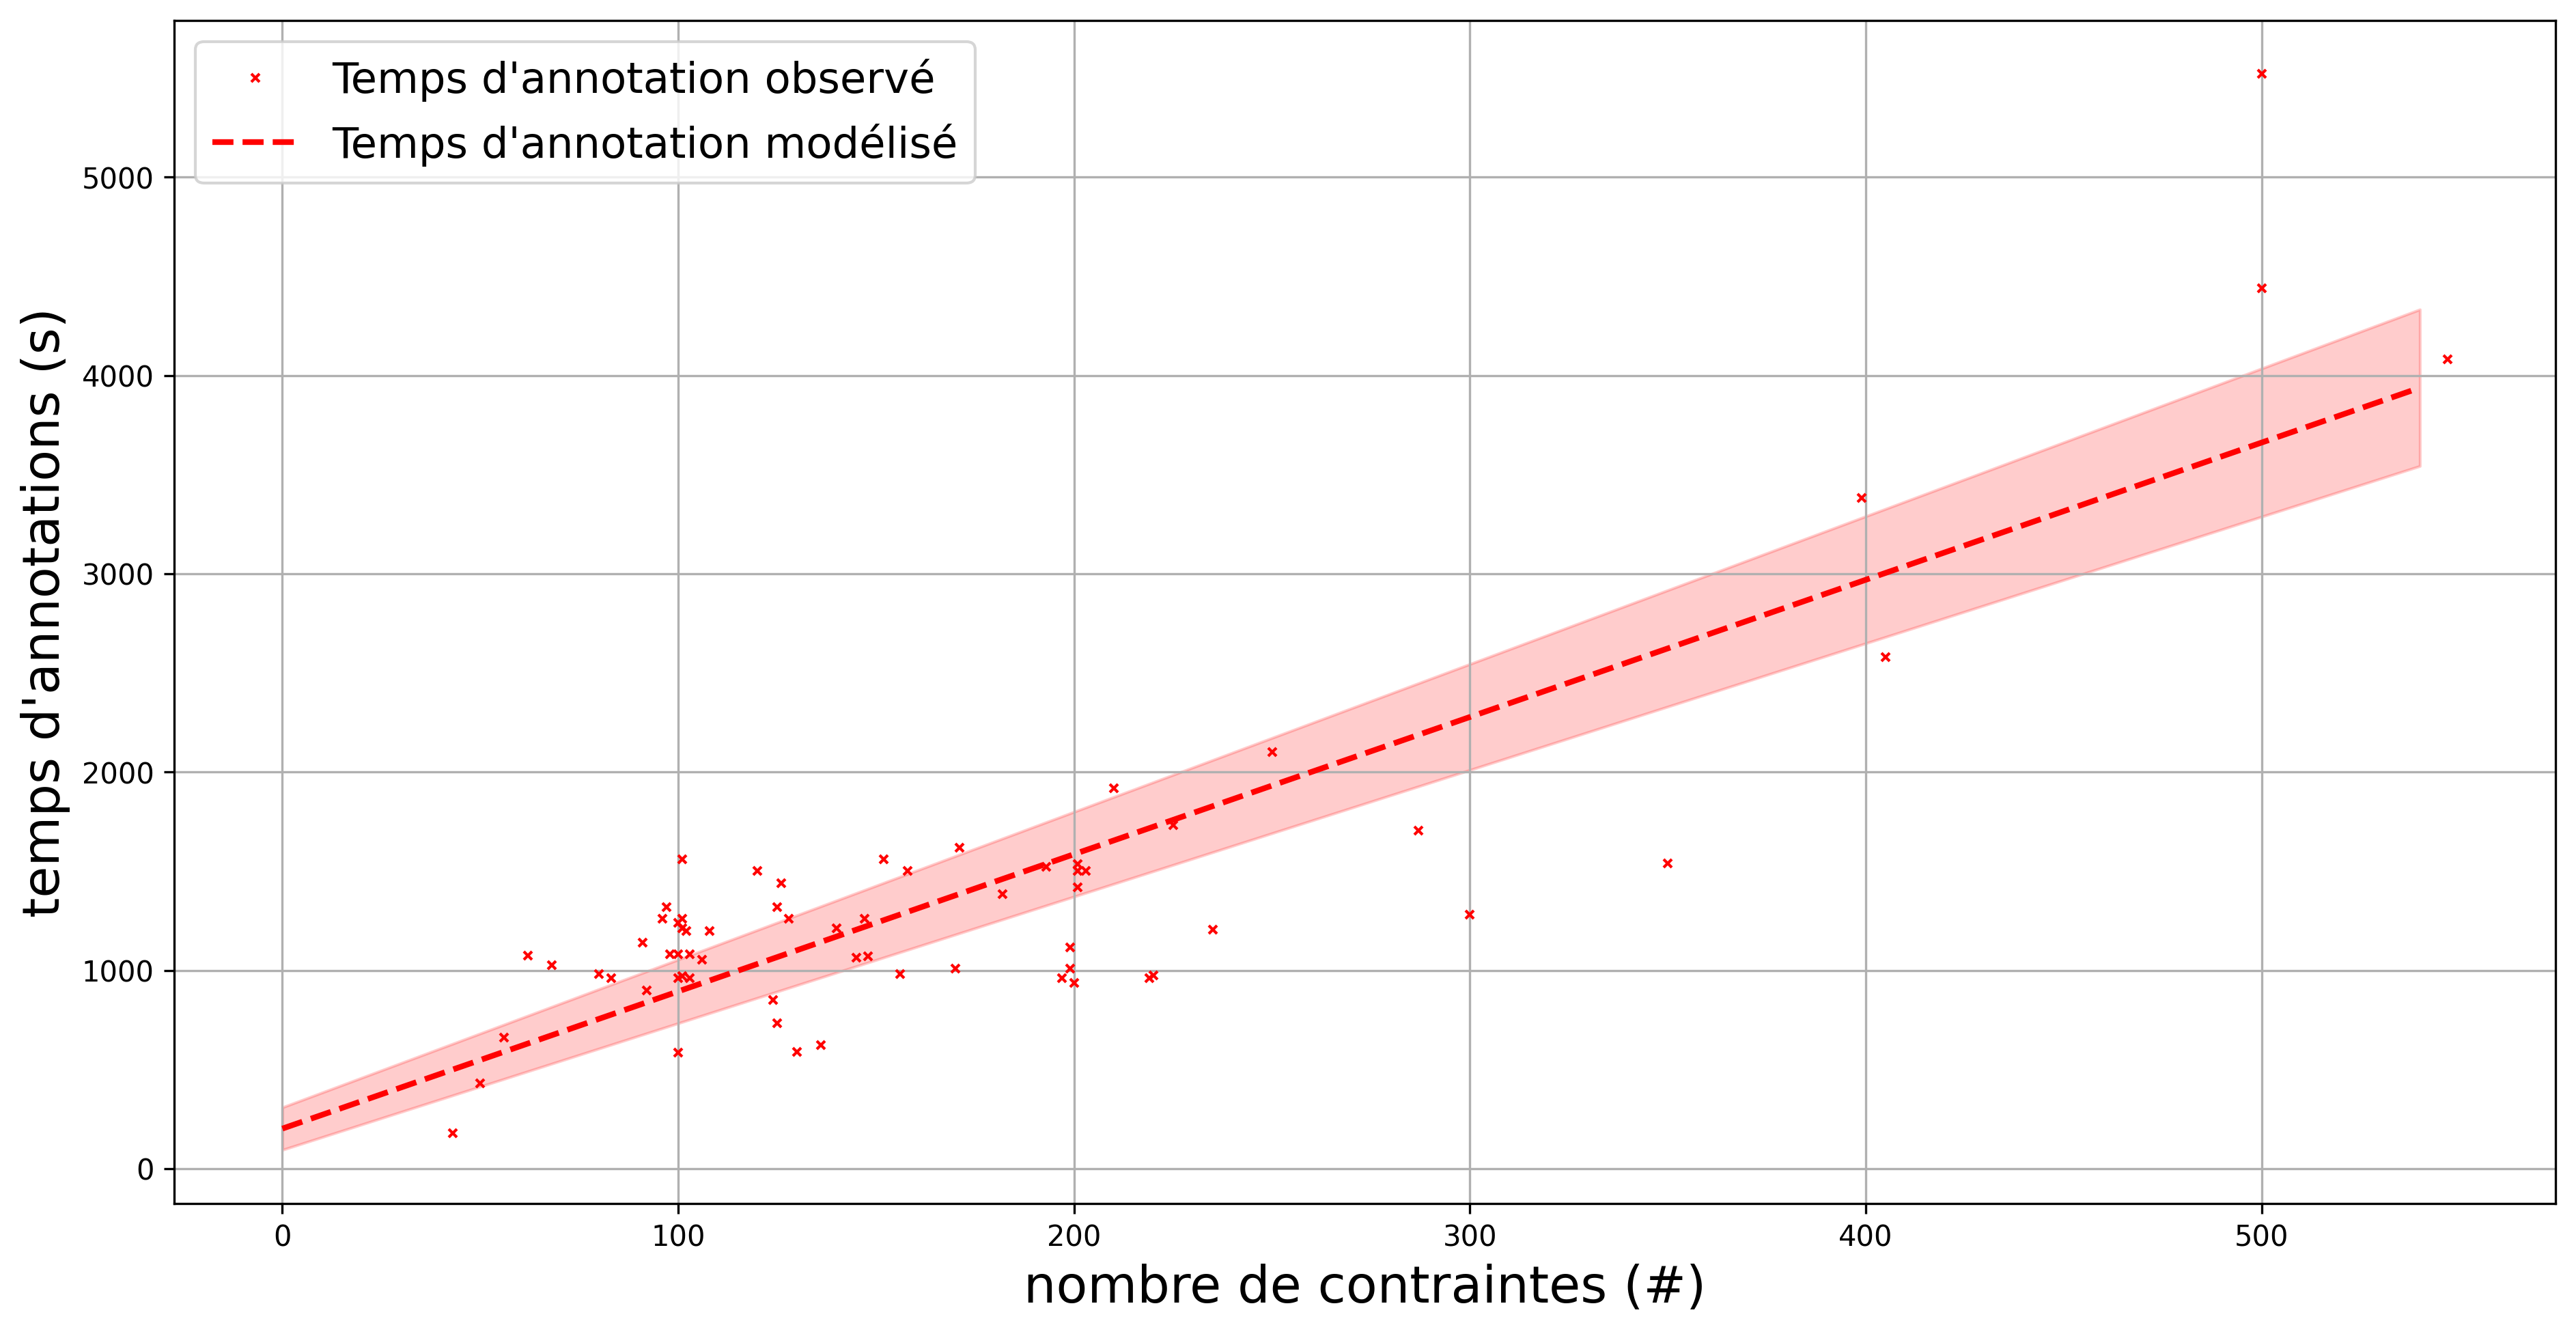
\includegraphics[width=\textwidth]{figures/etude-temps-annotation-1-modelisation-temps}
				\caption{Estimation du temps nécessaire (en secondes) pour annoter un lot de contraintes.}
				\label{figure:4.3.2-ETUDE-COUTS-TEMPS-ANNOTATION-SIMULATION}
			\end{figure}
			
			\todo[inline]{A REDIGER: quation du temps}
		
			\todo[inline]{A REDIGER: Description figure}			
			\begin{figure}[!htb]
				\centering
				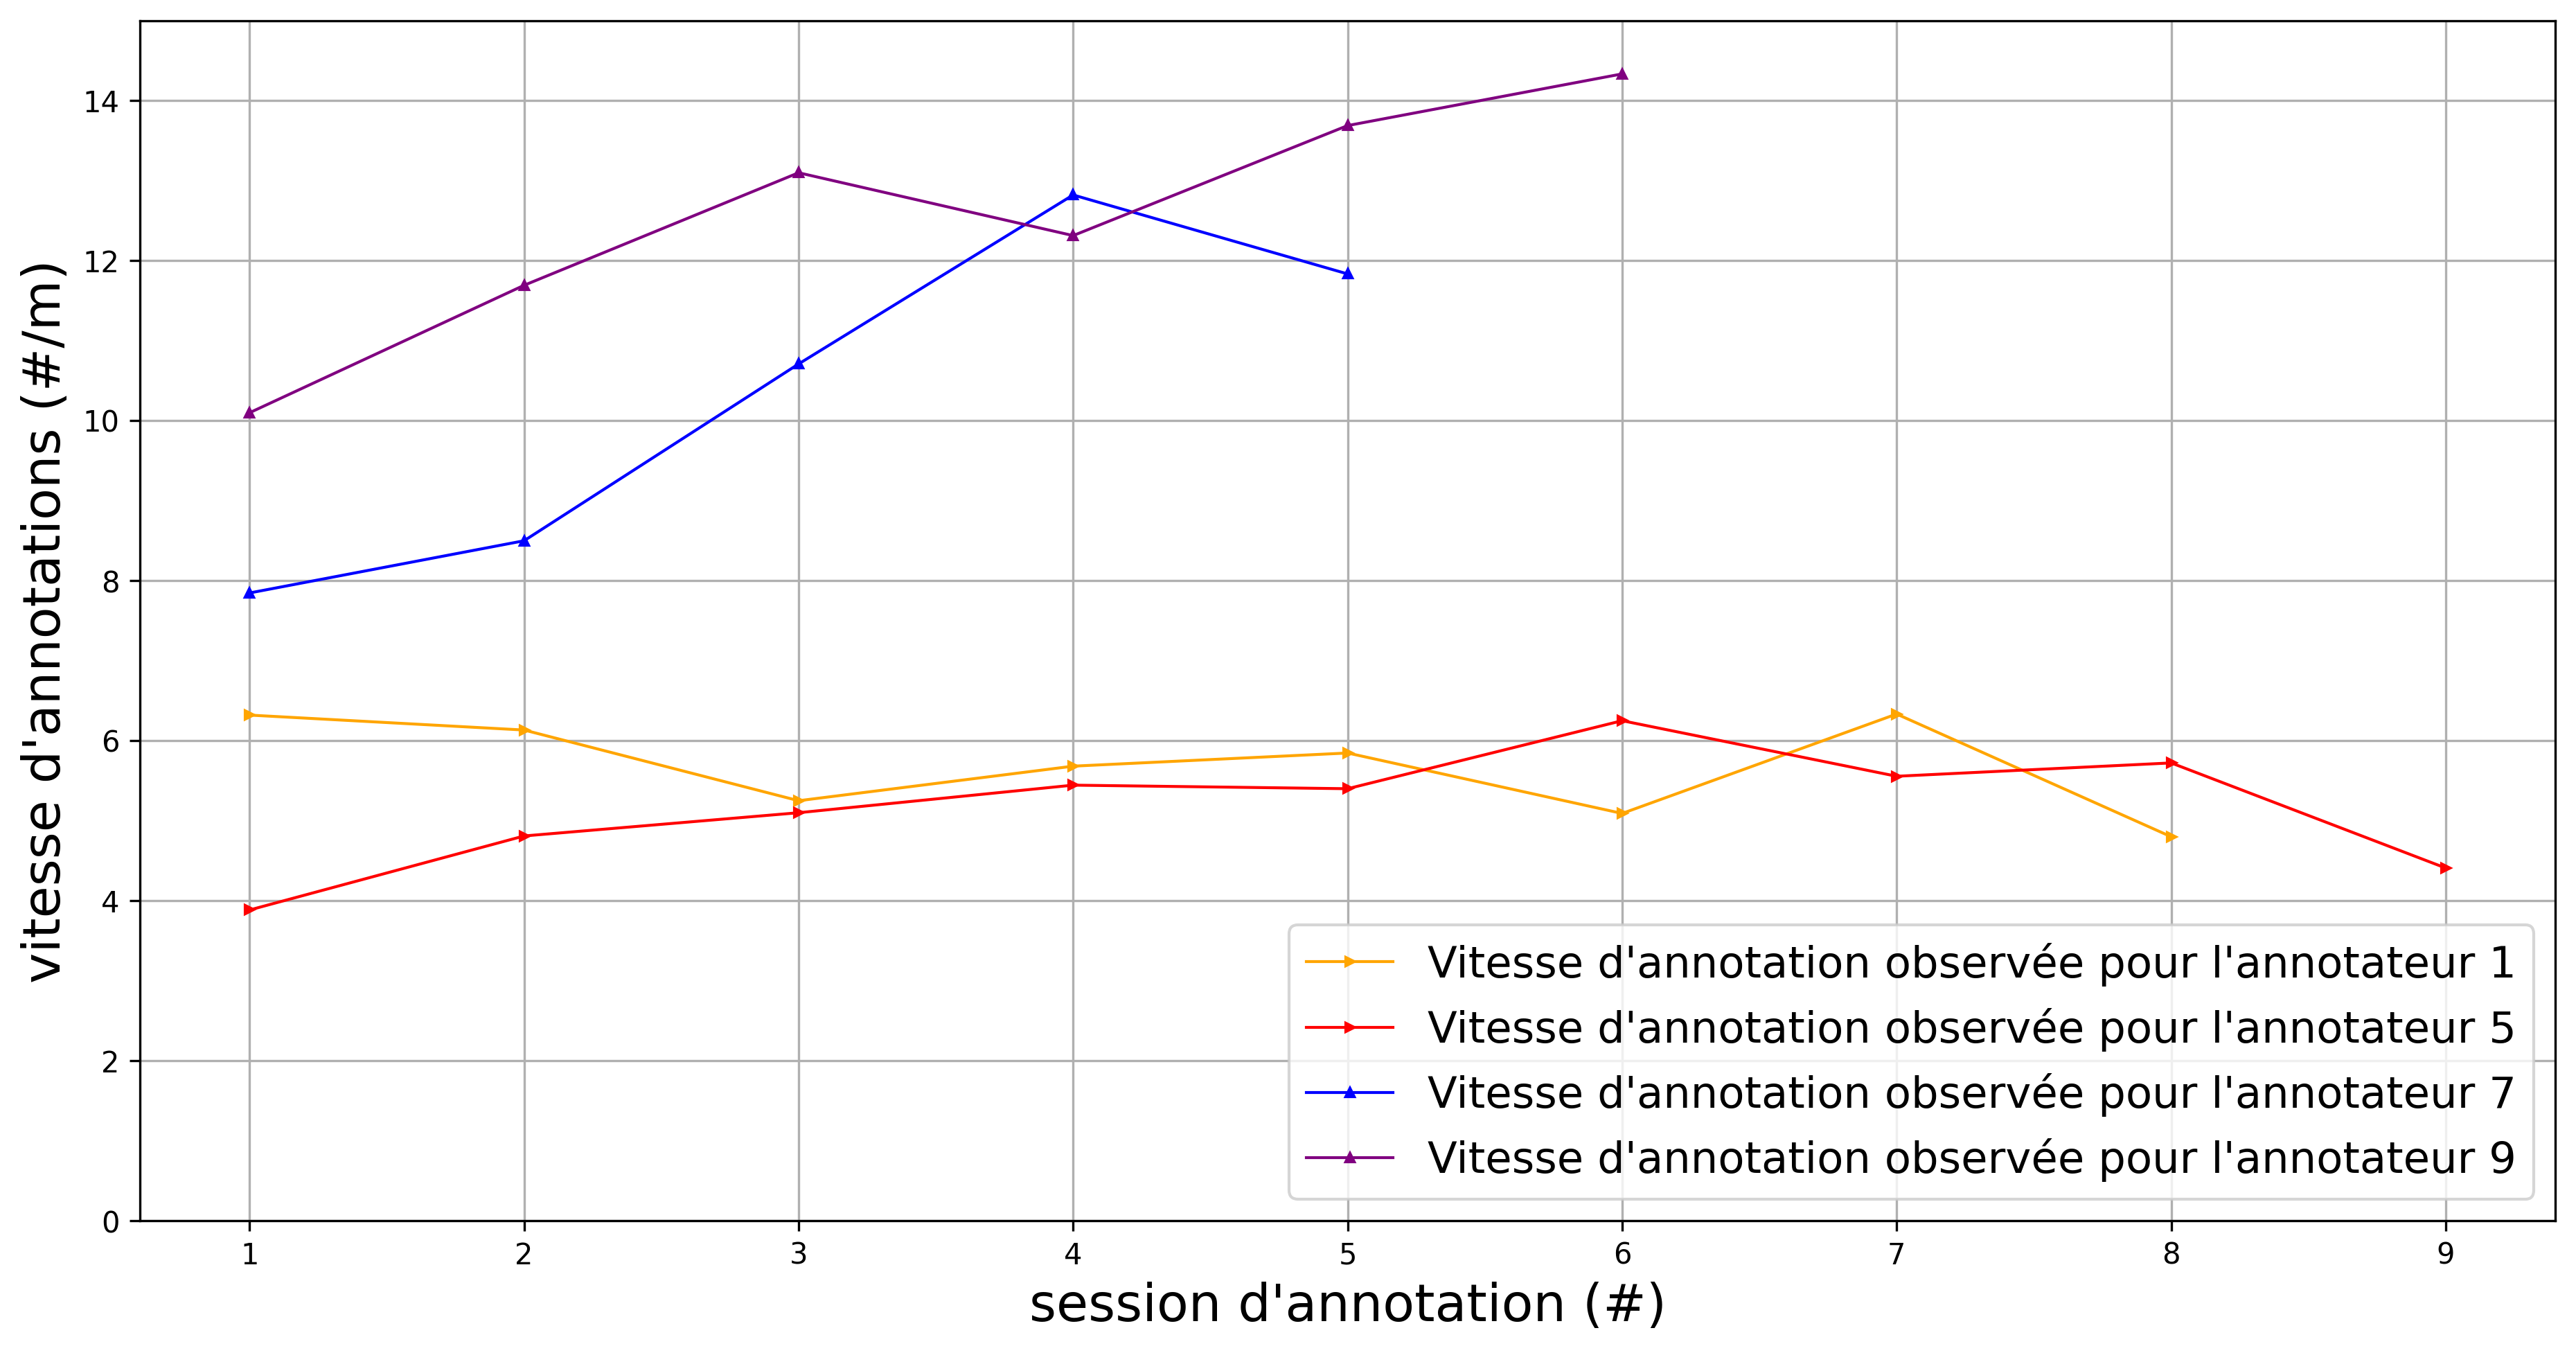
\includegraphics[width=\textwidth]{figures/etude-temps-annotation-3-etude-de-cas}
				\caption{Etude de cas d'évolution de la vitesse d'annotation de contraintes (en contraintes par minutes) en fonction des différentes sessions d'annotations}
				\label{figure:4.3.2-ETUDE-COUTS-TEMPS-ANNOTATION-EXEMPLE}
			\end{figure}

		%%% Discussion
		\subsubsection{Discussion}
		
			\todo[inline]{A REDIGER: Discussion temps moyen}
			\todo[inline]{A REDIGER: Discussion vitesse d'annotation}
	
	%%%
	%%% Subsection 4.3.3: Étude d'estimation du temps total d'un projet d'annotation
	%%%
	\subsection{Étude d'estimation du temps total d'un projet d'annotation}
	
		%%% Protocole expérimental.
		\subsubsection{Protocole expérimental}
			\todo[inline]{Description succincte du protocole expérimental dans l'encadré d'hypothèse ?}

		%%% Résultats
		\subsubsection{Résultats obtenus}

		%%% Discussion
		\subsubsection{Discussion}